\documentclass[USenglish]{tex/lipics-v2016}
\usepackage{stmaryrd} 
\usepackage{xspace,listings,url,framed,amssymb,
            hyperref,doi, mathtools,wrapfig,
            stmaryrd, graphicx, tikz, colortbl, xparse, etoolbox,
            pgffor, makecell, microtype}
            \usetikzlibrary{decorations.pathreplacing}

\usepackage[customcolors,norndcorners]{hf-tikz}
\usepackage{tex/mathpartir}
\usetikzlibrary{arrows}
\usetikzlibrary{shapes.geometric}
\usetikzlibrary{shapes.multipart}
\usetikzlibrary{positioning}
\usetikzlibrary{calc}
\usetikzlibrary{backgrounds}
\usepackage[inline]{enumitem}
\usepackage{epigraph}
\setlength{\epigraphrule}{0pt}
\renewcommand*{\textflush}{flushright}
\setlength{\epigraphwidth}{4in}
\newcommand{\code}[1]{{\tt #1}\xspace}
\newcommand{\FZ}[1]{\textbf{FZ: #1}}
%% Formatting
\newcommand{\EM}[1]{\ensuremath{#1}\xspace}
\newcommand{\xt}[1]{{\sf{#1}}}
\newcommand{\bt}[1]{\xt{\bf #1}}
\renewcommand{\b}[1]{\EM{\overline{#1}}}
\newcommand{\EMxt}[1]{\EM{\xt{#1}}}
\newcommand{\EMbt}[1]{\EM{\bt{#1}}}

%% Variables
\newcommand{\x}   {\EMxt x}
\newcommand{\n}   {\EMxt n}
\newcommand{\e}   {\EMxt e}
\newcommand{\m}   {\EMxt m}
\newcommand{\s}   {\EM{\sigma}}
\renewcommand{\t} {\EMxt t}
\newcommand{\ta}  {\EM{\tau}}
\renewcommand{\a} {\EMxt a}
\newcommand{\K}   {\EMxt K}
\renewcommand{\k} {\EMxt k}
\newcommand{\Kp}  {{\EMxt{K'}}}
\newcommand{\Kpp}  {{\EMxt{K''}}}
\newcommand{\Kppp}  {{\EMxt{K'''}}}
\newcommand{\ep}  {{{\EMxt{e'}}}}
\newcommand{\epp}  {{{\EMxt{e''}}}}
\renewcommand{\sp}{{{\EM{\s'}}}}
\newcommand{\spp}{{{\EM{\s''}}}}
\newcommand{\ap}  {\EM{\a'}}
\newcommand{\aE}[1]  {\EM{\a_{#1}}}
\newcommand{\app}  {\EM{\a''}}
\newcommand{\tp}  {\EM{ \t'}}
\newcommand{\tpp}  {\EM{ \t''}}
\newcommand{\C}   {\EMxt C}
\newcommand{\Cp}  {\EMxt{C'}}
\newcommand{\EC}   {\EMxt E}
\newcommand{\fd}  {\EMxt{fd}}
\newcommand{\md}  {\EMxt{md}}
\newcommand{\mdpp}  {\EM{\md'}}
\newcommand{\mt}  {\EMxt{mt}}
\newcommand{\mtp}  {\EMxt{mt'}}
\newcommand{\mtpp}  {\EMxt{mt''}}
\newcommand{\M}{\EMxt M}
\newcommand{\MN}  {\EMxt{M\,K}}
\newcommand{\MNargs}[1]  {\EMxt {M #1~K}}
\newcommand{\f}   {\EMxt f}
\newcommand{\fp}   {\EMxt{ f'}}
\newcommand{\E}   {\EM{\Gamma}}
\newcommand{\EE}   {\EM{\mathcal{E}}}
\newcommand{\any} {\EM{\star}}
\newcommand{\this}{\EMxt{this}}
\newcommand{\that}{\EMxt{that}}
\newcommand{\none}{\EM{\cdot}}
\newcommand{\D}   {\EMxt D}
\newcommand{\Dp}   {\EMxt{D'}}
\newcommand{\p}   {\EMxt p}
\newcommand{\np}{\n'}

\newcommand{\Get}[2]   {\EM{#1.#2()}}
\newcommand{\Set}[3]   {\EM{#1.#2(#3)}}
\newcommand{\Call}[3]  {\EM{#1.#2(#3)}}
\newcommand{\DynCall}[3]  {\EM{#1@#2(#3)}}

\newcommand{\New}[2]   {\EM{\new\;#1(#2)}}
\newcommand{\SubCast}[2]{\EM{<\hspace{-.6mm}{#1}\hspace{-.6mm}>\hspace{-1mm}\;{#2}}}
\newcommand{\ShaCast}[2]{\EM{\prec #1 \succ #2}}
\newcommand{\MonCast}[2]{\EM{\triangleleft\; #1 \triangleright #2}}
\newcommand{\BehCast}[2]{\EM{\blacktriangleleft #1 \blacktriangleright #2}}
\newcommand{\new}      {\EM{\bt{new}}}
\newcommand{\HT}[2]    {\EM{{#1}\!:{#2}}}
\newcommand{\Mdef}[5]  {\EM{ \HT{ #1( \HT{#2}{#3})}{#4}\;\{{#5}\}}}
\newcommand{\Mdefz}[3] {\EM{ \HT{ #1()}{#2}\;\{{#3}\}}}
\newcommand{\Mdefa}[4]  {\EM{ \HT{ #1( #2 )}{#3}~\{{#4}\}}}
\newcommand{\obj}[2]   { \EM{ #1\{#2\}}}
\newcommand{\alloc}[4] {\EM{#1\;#2  = \xt{alloc}(#3, #4)}}
\newcommand{\cast}[8]  {\EM{#6\;#7\;#8=\xt{#5 cast}(#1, #2, #3, #4)}}
\newcommand{\behcast}[7]  {\EM{\xt{behcast}(#1, #2, #3, #4)=#5\,#6\,#7}}
\newcommand{\moncast}[6]  {\EM{\xt{moncast}(#1, #2, #3, #4)=#5\,#6}}

\newcommand{\Alt}[1]   { &\B #1 \\}
\newcommand{\B}        {\EM{~|~}}
\newcommand{\bang}     {\EM{\xt{!}}}

\newcommand{\dispatch}[5] {\EM{#1\;#2 = \xt{disp}(#3,#4,#5)}}
\newcommand{\readf}[4]{\EM{\xt{read}(#1,#2,#3,#4)}}
\newcommand{\convert}[1]{\EM{\xt{cnvtMD}(#1)}}
\newcommand{\convertFD}[1]{\EM{\xt{cnvtFD}(#1)}}
\newcommand{\readfield}[4]{\EM{#1 = \xt{read}(#2,#3,#4)}}
\newcommand{\setf}[5] {\EM{\xt{write}(#1,#2,#3,#4,#5)}}
\newcommand{\Reduce}[6]   {\EM{{#1}~{#2}~{#3} \rightarrow {#4}~{#5}~{#6}}}
\newcommand{\ReduceA}[6]  {\EM{#1~#2~#3 } & \EM{\rightarrow #4~#5~#6}}
\newcommand{\Class}[3]    {\EM{\bt{class}\;#1\,\{\,#2~#3\,\}}}
\newcommand{\Ftype}[2]    {\EM{ \HT{#1}{#2} }}
\newcommand{\Fdef}[2]    {\EM{ \HT{#1}{#2} }}
\newcommand{\Mtype}[3]    {\EM{ \HT{#1(#2)}{#3}}}
\newcommand{\Type}[1]     {\EM{\{#1\}}}

\newcommand{\opdef}[2]    {\framebox[1.1\width]{#1} ~ #2\\}
\newcommand{\Map}[2]     {\EM{ #1[#2] }}
\newcommand{\Bind}[2]     {\EM{#1 \mapsto #2}}

\newcommand{\Sub}{\EM{<:}}
\newcommand{\OK}{\EM{~\checkmark}}
\newcommand{\SubE}[1]{\EM{<:_{#1}}}
\newcommand{\names}[1]{\EM{\xt{names}(#1)}}
\newcommand{\untyped}[1]{\EM{\xt{untyped}(#1)}}

\newcommand{\mnames}[1]{\EM{\xt{methName}(#1)}}
\newcommand{\fnames}[1]{\EM{\xt{fieldName}(#1)}}


\newcommand{\ConsSub}{\EM{\lesssim}}

\newcommand{\CondRule}[3]{ #3 &~ #2 \\}
\newcommand{\SuchRule}[3]{ #3 &~{\emph{s.t.}} #2 \\}
\newcommand{\EnvType}[5]{ \EM{#1\,#2\,#3\vdash #4 : #5}}

\newcommand{\IRule}[4][]{\inferrule*[lab={\tiny #2},#1]{#3}{#4}}
\newcommand{\HasType}[3]{ \EM{#1 (#2) = #3}}
\newcommand{\wrapper}[1]{\EM{\xt{wrap}(#1)}}
\newcommand{\spec}[4]{\EM{\xt{spec}(#1,#2,#3,#4)}}

\newcommand{\castfn}[4]{\text{cast}(#1,#2,#3,#4)}
\newcommand{\GenCast}[5]{#1~#2 \vdash #3 \hookrightarrow #4 \Uparrow #5 }
\newcommand{\AnaCast}[5]{#1~#2 \vdash #3 \Downarrow #5 \hookrightarrow #4}
\newcommand{\TransClass}[2]{\EM{ #1 \rightharpoonup #2 }}
\newcommand{\inv}[2]{\xt{invoke}(#1, #2)}
\newcommand{\classoff}[2]{\EM{\xt{mtypes}(#1,#2)}}
\newcommand{\classoffs}[3]{\EM{\xt{mtypes}(#1,#2,#3)}}
\newcommand{\mtype}[3]{\EM{\xt{mtype}(#1,#2,#3)}}
\newcommand{\wftype}[3]{\EM{\xt{wftype}(#1,#2,#3)}}

\newcommand{\field}[2]{\EM{\xt{field}(#1,#2)}}
\newcommand{\In}{\EM{\in}}

\newcommand{\T}{\EM{\xt T}}
\newcommand{\Cast}{Cast }
\newcommand{\fb}{\EM{\xt{f!}}}

\newcommand{\AND}{\EM{\wedge}}
\newcommand{\App}[2]{\EM{#1(#2)}}

\newcommand{\StrSub}[4]{\EM{#1~#2\vdash #3\Sub #4}}
\newcommand{\tmeet}[4]{\xt{tmeet}(#1,#2,#3,#4)}
\newcommand{\mmeet}[4]{\xt{mmeet}(#1,#2,#3,#4)}
\newcommand{\mtypes}[2]{\xt{mtypes}(#1,#2)}


\newcommand{\WFtype}[2]{\EM{#1\vdash#2 \OK}}
\newcommand{\WF}[4]{\EM{#1\,#2\,#3\vdash#4 \OK}}
\newcommand{\WFp}[3]{#1~#2~#3\OK}

\renewcommand{\P}{\EMxt P}
\newcommand{\Pp}{\EMxt{P'}}


\newcommand{\retype}[5]{\xt{retype}(#1,#2,#3,#4,#5)}
\newcommand{\htype}[3]{\EM{\xt{htype}(#1,#2,#3)}}
\newcommand{\ftypes}[4]{\xt{ftypes}(#1,#2,#3,#4)}
\newcommand{\typeof}[1]{\xt{typeOf}(#1)}
\newcommand{\classgen}[1]{\xt{classgen}(#1)}
\renewcommand{\S}{\EM{\tau}}
\newcommand{\Sp}{\EM{\tau'}}
\newcommand{\Spp}{\EM{\tau''}}
\newcommand{\EQ}{\EM{\equiv}}

\newcommand{\Dom}[1]{\EM{\xt{dom}(#1)}}
\newcommand{\fresh}[1]{\EM{#1~\xt{fresh}}}

\newcommand{\progtrans}[2]{#1 ~\hookrightarrow_p~ #2}
\newcommand{\classtrans}[3]{#1 \vdash #2 ~\hookrightarrow_c~ #3}
\newcommand{\methtrans}[4]{#1~#2 \vdash #3 ~\hookrightarrow_m~ #4}
\newcommand{\statictype}[2]{\xt{static}(#1,#2)}

\definecolor{Gray}{gray}{0.9}
\definecolor{vlightgray}{gray}{0.93}
\pagestyle{headings} 

\lstdefinelanguage{JavaScript}{
  keywords={typeof,new,true,false,instanceof,catch,function,return,null, 
    catch, switch, var, if, in, while, do, else, case, break},
  keywordstyle=\color{darkgray},
  ndkeywords={class,def,interface,export,boolean,throw,extends,implements,import,this},
  ndkeywordstyle=\color{darkgray}\bfseries,
  identifierstyle=\color{black},
  sensitive=false,  comment=[l]{//},  morecomment=[s]{/*}{*/},
  commentstyle=\color{gray}\ttfamily,  stringstyle=\color{gray}\ttfamily,
  morestring=[b]',  morestring=[b]",
  %backgroundcolor=\color{vlightgray},
  aboveskip=\medskipamount, %0em,
  belowskip=\medskipamount, %0em
  escapeinside={(*@}{@*)}
}
\lstset{
  language=JavaScript,  extendedchars=true,  basicstyle=\small\ttfamily,
  showstringspaces=false,   showspaces=false,  numberstyle=\small,
  numbersep=9pt,  tabsize=2, breaklines=true,  showtabs=false, captionpos=b
}

\begin{document}
\title{KafKa: Gradual Typing for Objects}
\titlerunning{Gradual Typing for Objects}
\author{Benjamin Chung, Paley Li, Francesco Zappa Nardelli \& Jan Vitek}
\affil{Northeastern University \& INRIA \& Czech Technical University}
\authorrunning{Chung, Li, Zappa Nardelli, Vitek}
\Copyright{Benjamin Chung, Paley Li, Francesco Zappa Nardelli and Jan Vitek}
\subjclass{F.3.3 Studies of Program Constructs}
\keywords{Gradual typing, object-orientation, language design,
type systems}

% Author macros::end %%%%%%%%%%%%%%%%%%%%%%%%%%%%%%%%%%%%%%%%%%%%%%%%%

%Editor-only macros:: begin (do not touch as author)%%%%%%%%%%%%%%%%%%%%%%%%%%
\EventEditors{Todd Milstein}
\EventNoEds{2}
\EventLongTitle{European Conference on Object Oriented Programming}
\EventShortTitle{ECOOP 2018}
\EventAcronym{ECOOP}
\EventYear{2018}
\EventDate{July 16--21, 2018}
\EventLocation{Amsterdam, Netherlands}
\EventLogo{}
\SeriesVolume{42}
\ArticleNo{12}
% Editor-only macros::end %%%%%%%%%%%%%%%%%%%%%%%%%%%%%%%%%%%%%%%%%%%%%%%


\maketitle

\begin{abstract} 
The enduring popularity of dynamically typed languages has motivated
research on \emph{gradual type systems} to allow developers to annotate
legacy dynamic code piecemeal. Type soundness for a program which contains a
mixture of typed and untyped code cannot mean the traditional absence of a class of
errors. While some errors will be caught at type-checking time, other errors
can only be caught as the program executes. After a decade of research
there are a number of competing approaches to providing gradual type
support for object-oriented languages. We introduce a framework for
comparing gradual type systems, combining a common surface language with
a core calculus to which the surface language can be translated. 
The core calculus  is strongly typed in order to highlight where dynamic
operations are required.  We illustrate our approach by translating
idealizations of four different approach to gradually typing objects into that core
calculus and discuss the implications of the respective designs.
\end{abstract}

\section{Introduction}

\epigraph{\small\vspace{-5mm}
   \it ``Because half the problem is seeing the problem''}

\vspace{-10mm}\noindent There never was a single approach to gradual
typing. The field was opened by two simultaneously
published papers. One, by Siek and Taha, typed individual Scheme terms using a
consistency relation, inserting casts based on type inference
\cite{SiekTaha06}. The other, by Tobin-Hochtstadt and Felleisen, described a
system allowing programmers to add types to individual modules, using
constraint solving to determine where casts were needed in untyped code~\cite{tf-dls06}. 
These two approaches set the tone for a decade of research.
Today, gradual type systems support a variety of languages, enforcement
mechanisms, and soundness guarantees; this degree of linguistic diversity is
not without consequence, however, as the very notion of what constitutes an
error remains unsettled.

The type system and semantics of a programming language are necessarily
tightly coupled;  each has to deal with the language's complexity. As a result,
the same gradual type system may seem very different when applied to two
different languages, an issue that shows up clearly with object-oriented
languages. Siek and Taha's first effort~\cite{SiekTaha07} presented a gradual
type system for an object-based. It related objects by
generalizing the notion of consistency~\cite{SiekTaha06} over structural
subtyping. The work had drawbacks, most notably in the handling of
mutable state and aliasing --- vital features of object-oriented languages.
Underlying each subsequent gradual type system are different design choices on how to
deal with those features.

The landscape of gradually typed object-oriented languages is rich. 
Consider some of the languages in this space:

\begin{itemize}
 \item Typed Racket: a rich gradual type system based on contracts.
 \item Gradualtalk: a variant of Smalltalk with contracts.
 \item C\#: a statically typed language with a dynamic type.
 \item Dart: a class based language with optional types.
 \item Hack: a statically typed variant of PHP that allows untyped code.
 \item Thorn: a language with both statically typed and untyped code.
 \item TypeScript: JavaScript with optional types.
 \item StrongScript: a variant of TypeScript with nominal types.
 \item Nom: a language supporting dynamic types and nominal typing.
 \item Reticulated Python: a family of gradual type systems for Python.
\end{itemize}

\noindent These languages differ in their type system and the associated run-time
enforcement strategy. There are four major approaches, labeled here
as optional, concrete, behavioral and transient. The \emph{optional}
approach, chosen by TypeScript, Dart, and Hack, amounts to static
type-checking followed by type-erasure.  Erroneous values flowing from
dynamically typed code to statically typed code will not be caught. The
\emph{concrete} approach, used in C\# and Nom, uses run-time subtype tests on
type constructors to supplement static typing.  While statically typed code
executes at native speed, values are dynamically checked 
at typed-untyped boundaries. The \emph{behavioral} approach of Typed Racket, Gradualtalk and
Reticulated Python monitors values to ensure that they behave in accordance
to their assigned types. Instead of checking higher-order and mutable values for static
type tags like concrete, wrappers ensures enduring conformance of values to their declared type.
The \emph{transient} approach, specific to
Reticulated Python, lies between concrete and behavioral; it adds type casts
but does so only for the top-level of data structures. Finally, Thorn and
StrongScript combine the optional and concrete approaches,
differentiating between types that are erased and types that are run-time
checked.

Static type systems are designed to capture some class of errors. For
gradual type systems, however, some errors cannot be ruled out before
execution as untyped code can violate type guarantees. The meaning of error
for a gradual type system therefore depends on how type guarantees are
enforced.  In other words, each gradual type system may catch different
``errors''.  We demonstrate this with a litmus test consisting of three
simple programs capable of distinguishing the four above mentioned
approaches.  The litmus test programs are statically well-typed, and are
``correct'' in the sense that they run to completion without error in an
untyped language. However, when executed under different gradual typing
systems, they produce different errors. For intuition, consider a call,
\EM{\x.\m()}, where \EM{\x:\C} and \C has a method \m returning a \D.  In
the concrete approach, this call is guaranteed to succeed. With behavioral,
the call will go through, but an error may be reported if \m return the
wrong value. In transient, the call is similarly guaranteed to go through,
but might return the wrong value and not produce an error.  Finally, in
optional, the call may get stuck if the object denoted by \x does not have a
method \m, and if the call succeeds, there is no guarantee that a value of
type \D will be returned.

\begin{wrapfigure}{r}{5cm}
\vspace{-6mm}
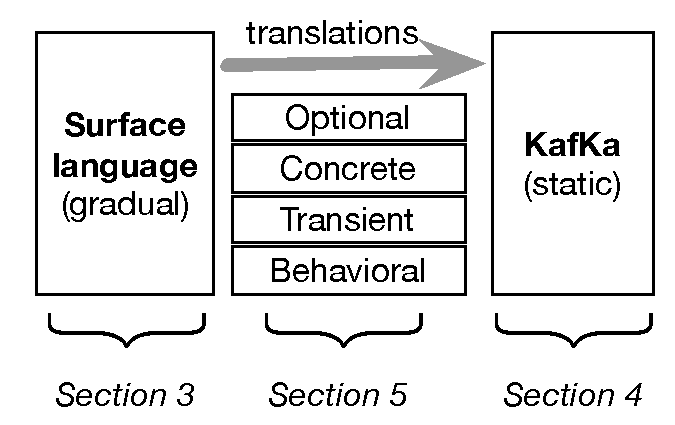
\includegraphics[width=5cm]{fig1}
%% \begin{center}\begin{tikzpicture}[node distance=3cm]
%% \node[draw,minimum height=3cm,minimum width=2cm] at (0,0) (S) {Source};
%% \node[draw,minimum height=3cm,minimum width=2cm,right=of S] (K) {\kafka};
%% %\node[draw,right=of K] (C) {CIL};
%% \draw [->] ([yshift=1cm]S.east) -- node[midway,above] {Optional} ([yshift=1cm]K.west);
%% \draw [->] ([yshift=0.33334cm]S.east) -- node[midway,above] {Transient} ([yshift=0.3334cm]K.west);
%% \draw [->] ([yshift=-0.33334cm]S.east) -- node[midway,above] {Behavioural} ([yshift=-0.3334cm]K.west);
%% \draw [->] ([yshift=-1cm]S.east) -- node[midway,above] {Concrete} ([yshift=-1cm]K.west);
%% %\draw [->] (K) -- (C);
%% \draw [decorate,decoration={brace,amplitude=10pt,raise=1pt},yshift=0pt] (S.north east) -- (K.north west) 
%%   node [above,midway,yshift=0.4cm] {Translations};
%% \node[label,below=0cm of S] {\footnotesize Section 3};
%% \node[label,below=0cm of K] {\footnotesize Section 4};
%% \draw [decorate,decoration={brace,amplitude=10pt,mirror,raise=1pt},yshift=0pt] (S.south east) -- (K.south west) 
%%   node [below,midway,yshift=-0.4cm] {\footnotesize Section 5};
%% \end{tikzpicture}\end{center}
\vspace{-7mm}\end{wrapfigure}

We propose to compare approaches to gradual typing for objects by translating
a gradually typed surface language to a target language, called \kafka. Our
surface language is a \emph{gradually} typed class-based object oriented
language, similar to Featherweight Java. \kafka is a \emph{statically} typed
class-based object calculus with mutable state. The key difference
between the two is the sound type system and casts of \kafka.
Where the surface language allows implicit coercions, \kafka requires
explicit casts to convert types. Casts come in two kinds:
\emph{structural casts} check if an object is a subtype of some type
\t, while \emph{behavioral casts} monitor that an object
behaves as if it was of some type \t. Translating from surface to target language
involves adding casts, the location and type of which depends on the gradual type system.

\noindent
This paper makes the following contributions:
\begin{itemize}  
  \item The design of a core calculus for gradual type systems for objects.
\item Translations of each gradual approach to the core calculus.
\item A litmus test comprised of three programs to tell apart the gradual
  type systems.
\item Supplementary material includes a mechanized proof of soundness of the
  type system of the core calculus and its proof-of-concept implementation
  on  .Net.
\end{itemize}

\noindent Our work does not address the question of performance of the
translations. Each of the semantics for gradual typing has intrinsic
performance costs, but these can be mitigated by compiler and run-time
optimizations which we do not perform. A departure from previous work
(e.g.~\cite{greenman18}) is that \kafka is statically typed.  By translating
to a statically typed core, we can clearly see where wrapper-induced dynamic
errors can occur. Another design choice is the use of structural subtyping
in \kafka. This is motivated by our desire to represent behavioral and
transient approaches that require structural subtyping. We do not foresee
difficulties either switching to a nominal type system or providing an
additional nominal subtype cast. Code and proofs are available from: {\small
  \url{github.com/BenChung/GradualComparisonArtifact}.}

\section{Background}

\epigraph{\vspace{-5mm}\small\it ``If you know the enemy and know yourself...''}

\vspace{-10mm}
\noindent The intellectual lineage of gradual typing can be traced back to
attempts to add types to Smalltalk and LISP. On the Smalltalk side, work on
the Strongtalk optional type system~\cite{Bracha93} led to Bracha's notion
of pluggable types~\cite{pluggabletypes}. For him, types exist solely to
catch errors at compile-time, never affecting the run-time behavior of
programs. An optional type system is \emph{trace preserving},
that is to say, if a term \e reduce to \a, then adding type annotations to
\e does not prevent it from reducing to that value~\cite{ecoop15}.  This property is valuable to
developers as it ensures that type annotations will not introduce errors, and
thus that adding types does not increase the testing burden!
Optional type systems in wide use include Hack~\cite{hack13},
TypeScript~\cite{BAT14} and Dart~\cite{dart13}.

Felleisen and his students have contributed substantially to gradual
typing. The Typed Scheme~\cite{tf-popl08} design that later became Typed
Racket is influenced by their earlier work on higher-order
contracts~\cite{ff-icfp02}. Typed Racket was envisioned as a vehicle for
teaching programming. Thus, being able to explain the source of errors and
avoiding surprises for beginning users were important considerations. Thus,
a value that flows in a variable of type \t, should behave as if it belonged
to that type throughout its lifetime.  Whenever a higher-order or mutable
value crosses a boundary between typed and untyped code, it is wrapped in a
contract that monitors the value's behavior.  If the value misbehaves, blame
can be assigned to the boundary that assigned it the type that was
violated. The granularity of typing is the module, thus a module is either
entirely typed or entirely untyped.  Typed Racket's support for objects was
described by Takikawa et al.~in~\cite{Takikawa:2012}.

Siek and Taha coined the term gradual typing in~\cite{SiekTaha06} as ``any
type system that allows programmers to control the degree of static checking
for a program by choosing to annotate function parameters with types, or
not.'' They formalized this idea in the lambda calculus augmented with
references. To make the type system a gradual one, they defined the type consistency
relation $\t \sim \tp$. If $\t \sim \tp$, then \t is consistent with \tp,
and can therefore be used implicitly where a \tp instance is expected.
This enables gradual typing, as $\any \sim \t$ for every $\t$ and vice versa,
allowing untyped values to be passed where typed ones are expected.
In~\cite{SiekTaha07} the authors extended this idea to an object calculus.
In order to do so, they combined consistency with structural subtyping,
producing consistent subtyping. With consistent subtyping, consistency can be used
when checking structural subtyping, allowing typed objects and untyped objects
to be mixed. 
To explore the design space, Reticulated Python~\cite{siek14} was given
three modes: the \emph{guarded}
mode behaves as Typed Racket with contracts applied to values.  The
\emph{transient} mode performs shallow subtype checks on reads and method
returns, only validating if the value obtained has matching method types.
The \emph{monotonic} mode is fundamentally different from any of the
previous approaches. Monotonic cast updates the type 
of values in place by replacing some of the occurrences of \any with more
specific types, these updates propagate recursively through the heap until
a fixed point is reached.

Other noteworthy systems include Gradualtalk~\cite{GS13}, C\#
4.0~\cite{Bierman10}, Thorn~\cite{oopsla09}, Nom~\cite{Muehlboeck2017} and
Strong\-Script~\cite{ecoop15}. Gradualtalk is a variant of Smalltalk with
Felleisen-style contracts and mostly nominal type equivalence (structural
equivalence can be specified on demand, but it is rarely
used). C\# 4.0 adds the type {\sf dynamic} to C\# and adds dynamically resolved
method invocation. Thus C\# has a dynamic sublanguage that allows developers
to write unchecked code, working alongside a strongly typed sublanguage in
which values are guaranteed to be of their declared type.  The
implementation replaces \any by the type {\tt object} and adds casts where
needed.  Thorn and StrongScript extend the C\# approach with the addition of
optional types (called {\em like types} in Thorn).  Thorn is implemented by
translation to the JVM. StrongScript translate to an extended version of
V8. The presence of concrete types means that the compiler can optimize code
(unbox data and in-line methods) and programmers are guaranteed that type
errors will not occur within concretely typed code. Nom is similar to Thorn
in that it is nominal and follows the concrete approach.

\newcommand{\rot}[1]{\rotatebox{80}{#1}\hspace{-10px}}
\newcommand{\X}{\EM{\bullet}}
\newcommand{\XX}{\EM{\bullet^{2}}}
\newcommand{\XY}{\EM{\bullet^{1}}}

\begin{figure}[!t]
  \center
  {\footnotesize
\begin{tabular}{r|lllllllllllllr}
 & & \rot{Nominal}
  & \rot{Optional}
  & \rot{Concrete}
  & \rot{Behavioral}
  & \rot{Class based}
  & \rot{First-class Class}
  & \rot{Soundness claim}
  & \rot{Unboxed prim.}
  & \rot{Subtype cast}
  & \rot{Shallow subtype cast}
  & \rot{Behavioral cast}
  & \rot{Blame}
  & \rot{Pathologies}
  \\
Dart         &&\X &\X &   &   &\X &   &    &    &\X &   &   &   &  - 
\\\hline
Hack         &&\X &\X &   &   &\X &   &    &    &\X &   &   &   &  -  
\\\hline
TypeScript   &&   &\X &   &   &\X &   &    &    &   &   &   &   &  -  
\\\hline
C\#          &&\X &   &\X &   &\X &   &\XX & \X &\X &   &   &   &  -  
\\\hline
Thorn        &&\X &\X &\X &   &\X &   &\XX & \X &\X &   &   &   & 0.8x
\\\hline
StrongScript &&\X &\X &\X &\X &\X &   &\XX &    &\X &   &\X &   & 1.1x   
\\\hline
Nom 		 &&\X &   &\X &   &\X &   &\XX & \X &\X &   &   &   & 1.1x
\\\hline
Gradualtalk  &&\XY&   &   &\X &\X &   & \X &    &   &   &\X &\X &  5x
\\\hline
Typed Racket &&   &   &   &\X &\X &\X &\X  &    &   &\X &\X &\X & 121x 
\\\hline
Reticulated Python    \\
\it Transient&&   &\X &   &   & \X &  & \X &    &   &\X &   &\X & 10x \\
\it Monotonic&&   &   &   &\X & \X &  & \X &    &   &   &\X &\X &  27x\\
\it Guarded  &&   &   &   &\X & \X &  & \X &    &   &   &\X &\X &  21x\\
\end{tabular}}
  \caption{Gradual type systems. (1) Opt.~structural constraints. (2)
    Typed expressions are sound.}\label{over}
\end{figure}

\figref{over} reviews gradual type systems for objects.  All
languages are class-based, except TypeScript which has both classes and
JavaScript objects. While that choice is not
crucial; classes are useful as a source of type declarations.
Most languages build subtyping on explicit subtype declarations -- nominal subtyping -- rather
than on structural similarities.  TypeScript uses structural subtyping, but
does not implement a run-time check for it. Anecdotal evidence suggests
that TypeScript could by switched to nominal subtyping with little effort, as
was done for StrongScript~\cite{ecoop15}.  While
nominal subtyping leads to more efficient type casts, Reticulated Python's
subtype consistency relation is fundamentally structural; it would be nonsensical to
use it in a nominal system. For Racket, the heavy use of
first-class classes and class generation naturally leads to structural
subtyping as many of the classes being manipulated have no names and arise
during computation.

The optional approach is the default for Dart, Hack and TypeScript.
Transient Reticulated Python allows any value to flow in a field regardless
of type annotations, leading to its ``open world'' soundness
guarantee~\cite{siek14}.  In Thorn, Nom and C\#, primitives are concretely
typed; they can be unboxed without tagging.  The choice of casts follows
from other design decisions. The concrete approach naturally tend to use
subtype tests to establish the type of values. For nominal systems, there
are highly optimized algorithms. Shallow casts are casts that only check the
presence of methods, but not their signature. They are used by Racket and
Reticulated Python to ensure some basic form of type conformance.  Behavioral casts are
used when information such as a type or a blame label must be associated
with a reference or an object.

Blame assignment is a topic of investigation in its own right. Anecdotal
evidence suggests that the context provided by blame helps developers
pinpoint the provenance of errors. In the same way that a Java stack trace
identifies the function that went wrong, blame identifies where a type assertion
came from. This is especially important in behavioural gradual type systems,
as type assertions become wrappers which can propagate through the heap. Blame
identifies where a failing wrapper came from, a task that would otherwise require
extensive backtracking debugging. Unlike stack traces, which have little run-time cost,
blame tracking has a cost due to its meta-data. Blame information has to be
stored whenever a wrapper is applied and is believed
to cause substantial slowdowns. However, this has not been measured in detail.
We are primarily concerned with where the error arises, rather than what information
is included in the error, thus we do not consider blame further.

The last column of \figref{over} lists self-reported performance
pathologies.  These numbers are not comparable as they refer to different
programs and different configurations of type annotations. They are not
worst case scenarios either; most languages lack a sufficient corpus of code
to conduct a thorough evaluation.  Nevertheless, one can observe that for
optional types no overhead is expected, as the type annotations are erased
during compilation. Concrete types insert efficient casts, and lead to code
that can be optimized.  The performance of the transient semantics for
Reticulated Python is a worst case scenario for concrete types -- i.e. there
is a cast at almost every call. Finally, languages with behavioral casts are
prone to significant slow downs. Compiler optimizations for reducing these
overheads are an active research topic~\cite{richards-bettermono,OnlyMostly}.  
Languages such as C\#, Nom, Thorn, and Strong\-Script are designed so that
the performance of fully typed code is better than untyped code, and so that
mixed code performs well thanks to the relatively inexpensive nominal subtype tests.


In contemporary work, Greenman and Felleisen describe three approaches to
\emph{migratory typing} in the context of a lambda calculus extended with
pairs and primitive values~\cite{greenman18}. Their \emph{natural embedding}
corresponds to the behavioral approach, the \emph{erasure embedding} is the
optional approach, and the \emph{locally-defensive embeddeding} is
transient. They do not consider the concrete approach nor do they support
objects, mutable state or subtying. They give performance results for a
non-optimizing implementation of the embeddedings, the results are as
expected: behavioral has extreme worst cases and locally-defensive
significantly slows down fully-typed programs. While they do not evalute
object-oriented programs, these are unlikely to fare better.

%%%%%%%%%%%%%%%%%%%%%%%%%%%%%%%%%%%%%%%%%%%%%%%%%%%%%%%%%%%%%%%%%%%%%%%%%%%

\section{A Family of Gradually Typed Languages and their Litmus Test}\label{litmustest}

\epigraph{\vspace{-4mm}\small\it ``There is no perfection only life''} 

\vspace{-10mm}
\noindent
There is no single, common, notion of what constitutes an erroneous gradually
typed program---a consequence of the varied enforcement strategies. The choice
of enforcement strategy is reflected in the semantics of the language,
which, in turn, implies that developers have to understand the details of
that strategy to avoid run-time errors.  This also
means that it is possible to differentiate between approaches by simply
observing the run-time errors that each type system produces. We propose a
litmus test consisting of three programs whose execution depends on which
gradual type system is in use. Each of these programs is statically 
well-typed and runs without error when executed with a purely dynamic semantics.
However, this varies as we use different semantics for gradual typing.
We start by presenting a common surface language in which we can
express our programs, and then explain why the various approaches to gradual
typing yield different run-time errors.

\subsection{A Common Surface Language}

\begin{figure}[!t]\hrulefill

\small
\vspace{5mm}

{\bf Syntax:}\\[3mm]

\begin{tabular}{ll}
\begin{minipage}{6cm}\begin{tabular}{@{}l@{~}l@{}l@{}l@{}l@{}l@{}l@{}l}
\k~::=~ \Class \C {\fd[1]..}{\md[1]..} \qquad
\md~::=~\Mdef\m\x\t\t\e\qquad
\fd~::=~ \Fdef\f\t\qquad
\t~::=~ \any \B \C\\[3mm]
\e~::=~\x\B\this\B\FRead\f\B\FWrite\f\e\B\Call\e\m\e\B\New\C{\e[1]..}
\end{tabular}\end{minipage} 
\end{tabular}

\vspace{5mm}


{\bf Typing expressions:}\\[-6mm]

\begin{mathpar}
\Rule{STG-VAR}{~\\\\ 
  \HasType \Env\x\t
}{
  \EnvTypeS \Env\K\x\t
}

\Rule{STG-GET}{
  \HasType \Env\this\C \\\\  \Fdef\f\t \in \App\K\C
}{
  \EnvTypeS \Env\K{\FRead\f}\t
}    

\Rule{STG-SET}{
  \HasType \Env\this\C \quad \Fdef\f\t \in \App\K\C \\\\
  \EnvTypeS \Env\K\e\tp \quad  \ConvertE\K{s}\tp\t
}{
  \EnvTypeS \Env\K{\FWrite\f\e}\t
}    

\Rule[width=15em]{STG-CALL}{
  \EnvTypeS \Env\K\e\any \\\\ \EnvTypeS \Env\K\ep\t 
}{
  \EnvTypeS \Env\K{\Call\e\m\ep}{\any}
}    

\Rule[width=15em]{STG-CALL}{
  \EnvTypeS \Env\K\e\C \quad \EnvTypeS \Env\K\ep\t \\\\
  \Mtype \m{\t[1]}{\t[2]}\in \App\K\C  \quad
  \ConvertE\K{s}\t{\t[1]}
}{
  \EnvTypeS \Env\K{\Call\e\m\ep}{\t[2]}
}   

\Rule{STG-NEW}{
  \Ftype{\f[1]}{\t[1]}.. \in \App\K\C \\\\
  \EnvTypeS \Env\K{\e[1]}{\tp[1]}..\quad \ConvertE\K{s}{\tp[1]}{\t[1]}..
}{
  \EnvTypeS \Env\K{\New\C{\e[1]..}}\C
}
\end{mathpar}


{\bf Convertibility:}\\[-6mm]
  
\begin{mathpar}
\Rule{SUB}{ \SSub\emptyset\K\t\tp}{ \ConvertE\K{s}\t\tp }
    
\Rule{TOA}{~ }{ \ConvertE\K{s}\t\any}
    
\Rule{ANYC}{~}{ \ConvertE\K{s}\any\t }
\end{mathpar}


{\bf Subtyping:}\\[-6mm]

\begin{mathpar}
\Rule{SAss}{  }{  \StrSub \M\K \any\any }

\Rule{SAss}{ \C \Sub \D \in \M }{  \StrSub \M\K \C\D }

\Rule{SRec}{
\M'=\M~\C\Sub\D\\\\\md\in\App\K\D\implies\mdp\in\App\K\C~.~\StrSub{\M'}\K\md\mdp
}{
 \StrSub \M\K \C \D 
}

\Rule{SMet}{
  \StrSub \M\K{\tp[1]}{\t[1]} \qquad \StrSub \M\K{\t[2]}{\tp[2]}
}{
 \StrSub\M\K{\Mdef\m\x{\t[1]}{\t[2]}\e}{\Mdef\m\x{\tp[1]}{\tp[2]}\ep}
}
\end{mathpar}

\hrulefill
\caption{Surface language syntax and type system (extract).}\label{slts}
\end{figure}

To normalize our presentation, we use a single surface language for all
four of the gradual type systems under study. The surface language is  a
\emph{gradually} typed object calculus without inheritance, method overloading
or explicit type cast operations. \figref{slts} gives its syntax and an
extract of its static semantics. The distinctive feature of the calculus  is
the presence of type \any\,-- the dynamic type. A variable of type \any can
hold any value, an invocation of a method with receiver of type \any is
always statically well-typed, and an expression of type \any can appear
anywhere within a typed program.

This dynamic type lets us convert our otherwise statically typed language to
being gradually typed. If a well-typed program does not use \any then it
will not get stuck on method invocation.  A program where all variables are
annotated as \any is fully dynamic and any given invocation may get
stuck. Gradual typing comes into play when an expression of type \any occurs
as an argument to a method that expects some other type \C and conversely
when an argument of type \C is passed to a method that expects \any. The
static type system of the surface language allows such implicit coercions --
using the \emph{convertibility} relation -- but run-time checks may be
inserted to catch potential type mismatches. We formalize the
semantics of this system later; here, we appeal to the reader's intuition.

Before presenting the litmus tests, some details about the type system of the
surface language may prove helpful. The subtyping relation is structural
with the Amber rule~\cite{cardelli1985amber} to enable recursion. \StrSub\M\K\C\D holds if class
\C has (at least) all the methods of class \D and the arguments and return
types are related by subtyping in the usual contra- and co-variant way; the
class table \K holds definitions of all classes and \M is a helper for
recursion. One noteworthy feature of subtyping is that the fields of objects
do not play a role in deciding if classes are subtypes. Following languages
like Smalltalk, fields are encapsulated and can only be accessed from within their
defining object. Syntactically, field reads and writes are limited to
the self-reference \this. 

The static type-checking rules are standard with two exceptions:
Method invocation is always allowed when the receiver \e is of 
type \any; therefore \EM{\e.\m(\ep)} has type \any if the argument
can have type \any. Secondly, we introduce a notion of convertibility, 
which allows the mixing of static and dynamic types. 
Convertibility is used when statically typed and dynamically typed terms
interact. The convertibility relation, written $\ConvertE\K s\t\tp$, states
that type $\t$ is convertible to type $\tp$ in class table \K.  It
is used both for up-casting and for conversions of \any to non-\any types.
$\ConvertE\K s\t\tp$ holds when $\t\Sub\tp$, this allows up-casts. The
remaining two rules allow implicit conversion to and from the dynamic type.
To avoid collapsing the type hierarchy, convertibility is not transitive.
It is through convertibility that our surface language becomes gradual; the
implicit conversions that it allows break soundness of the type system.


\subsection{Litmus}

Using three different programs, we can differentiate between four gradual
type systems. The litmus test is shown in \figref{litmus} and its
constituent programs are written in our surface language.  Each of these
programs consists of a class table and an expression whose evaluation in
the context of the class table determines if the litmus test succeeds or
fails.

The programs are designed to induce errors.  This is done via the
construction of an untyped value that violates the type guarantees of some
systems, but not others.  At heart, these programs can be summarized by the
typed/untyped boundaries that are crossed by an object. Let us use the
notation $\C ~\vert_{\,\t}$ to denote that an object of class \C passes
through a type boundary that expects it to be of type \t. For example,
if method \m expects an argument of type \t, a method call $\e.\m(\ep)$ would
induce the boundary $\ep ~\vert_{\,\t}$. 
In program {\bf L1}, we have \[\A ~\vert_{\,\any} ~ \vert_{\,\I}\] an instance of 
class \A is first implicitly converted to \any and then to \I; in this program
classes \A and \I are unrelated by subtyping. In {\bf L2}, the same sequence
of conversions is applied
\[\A~ \vert_{\,\any} ~ \vert_{\,\I}\] but this time \A and \I both have a
method \m, but the methods have incompatible argument types.  Lastly, in
{\bf L3} we start by converting a \C to \any and then to \E
and finally back to \any.
\[\C~ \vert_{\,\any}~\vert_{\,\E}~\vert_{\,\any}\]
The resulting value is then used to call  method \m with argument of class \C.
This correct as method \m in \C does expect an
argument of that type. If the object was an instance of \E instead, the call
would not be legal because \E's method \m expects a class \D as argument.

\begin{figure}[!h] 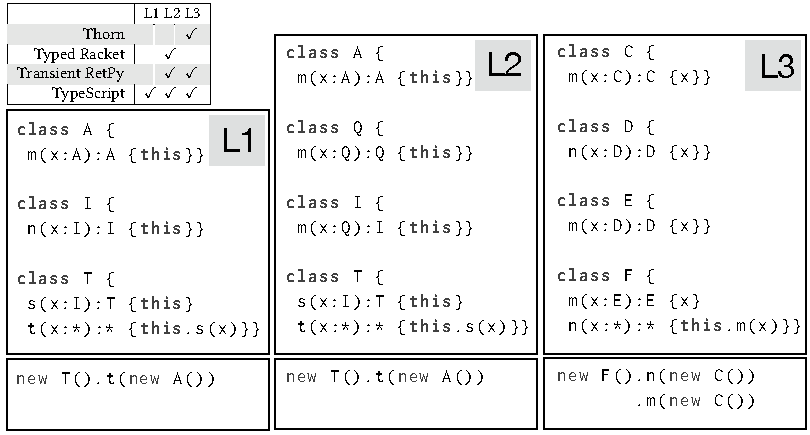
\includegraphics[width=.95\columnwidth]{../figures/litm}
  \caption{Gradual typing litmus test.}\label{litmus}
\end{figure}

\noindent We will use this litmus test to differentiate between four different
gradual type systems:
\vspace{2mm}\noindent
{\bf Optional.~} An optional gradual type system simply erases all of the
type annotations at run-time; all three programs run to completion without
error.

\vspace{2mm}\noindent {\bf Concrete.~} The guarantee provided by the
concrete approach is that all implicit conversion imply a run-time subtype
check.  This causes all three programs to fail. {\bf L1} and
{\bf L2} fail on a subtype test \StrSub{}\K\A\I.  {\bf L3} fails on the
subtype test \StrSub{}\K\C\E.

\vspace{2mm}\noindent {\bf Behavioral.~} The behavioral approach does allow
conversion from \any to \C if the actual value is ``structurally''
compatible to \C and if, after that, the value ``behaves'' as if it was an
instance of \C.  This is checked by a run-time shallow subtype cast that
looks at method names, and by a wrapper that monitors further interactions.
{\bf L1} is fails at run-time because \A does not have the method \xt n expected by
\I. {\bf L2}, however, executes without error because \A has the method \m
expected by \I (argument types are not checked). {\bf L3} fails, the
instance of \C has been applied a wrapper that checks it behave as if it was
an \E.  When method \a is called with a \C as argument, the wrapper notices
that \E's method \a expects a \D and that \C and \D are not compatible.

\vspace{2mm}\noindent {\bf Transient.~} The transient approach has a weaker
guarantee. It retains the shallow structural checks at casts of the
behavioral approach, but does not wrap values. Transient fails {\bf L1}, for
the same reason as the other two type systems, and passes {\bf L2}, for the
same reason as behavioral.  {\bf L3} succeeds because transient forgets that
the \C object was converted to \E.

\subsection{Discussion}

The litmus tests also capture the behavior of real languages. These three
programs have been expressed in TypeScript (optional), StrongScript
(concrete), Typed Racket (behavioral) and Reticulated Python
(transient).\footnote{\small
  \url{github.com/BenChung/GradualComparisonArtifact/examples}} Those
implementations have the same errors.

What the litmus tests show is that a precise understanding of the semantics of
gradually typed languages, their run-time enforcement machinery, is crucial
for developers to know when their programs is ``correct.'' They must
understand when the gradual type system will produce an error. In
the litmus test, all errors are false positives, since none of these programs ever
actually performs an invalid operation. This underlines the fact that in 
gradually typed language, false type specifications can create run-time
errors just as faulty code could. Thus, type annotations must be audited 
and tested just like code.

The different approaches induce usability trade-offs. One way to
contextualize this is with the gradual guarantee of Siek et
al~\cite{GradualGuarantee}. Put informally, the gradual guarantee states
that if there exists a static type assignment to an untyped program, any
partial assignment of those types will still execute successfully. The
optional approach trivially fulfills this guarantee.  However, this comes at
the cost of soundness. Transient likewise satisfies the gradual
guarantee~\cite{Vitousek2017}, as it only checks top-level structure of
values at type boundaries. Unlike optional, transient does guarantee that
typed calls will succeed; however, the call may produce a dynamic error if
the receiver is of the wrong type (even when called from a typed context),
or it can return an ill-typed value to a typed call site (which is checked
by the caller). The behavioral approach also fulfills the gradual guarantee,
as it will only check argument and return types when wrappers are
invoked. However, typed function calls might fail still if they call an
untyped function that returns the wrong value. Finally, the concrete
approach provides an absolute guarantee that every typed function call will
be successful. However, this comes at the expense of the gradual guarantee
-- partially typed classes are not compatible with more-or-less typed ones
under the concrete approach.  The gradual guarantee is incompatible with
subtyping. Suppose a program were to rely on the judgment $\{m(\C):\D\} <:
\{m(\C):\D\}$.  No one of these \C types can be removed while retaining the
subtyping relationship. To overcome this, Reticulated Python augments
subtyping with the aforementioned consistency relation.  Consistent
subtyping admits $\{m(\any):\D\} <: \{m(\C):\D\}$.  This increases the
number of programs accepted by the static type system. However, consistent
subtyping is not used by the run-time semantics, and is fundamentally
incompatible with the concrete approach (any use of consistent subtyping is
guaranteed to fail).  We omit consistent subtyping from our surface
language.

An alternative to the gradual guarantee is presented in the approaches
taken by Thorn or StrongScript. They have three kinds of types, \any (dynamic),
\C (concrete), and \xt{like} \C (optional), combining the concrete and
optional approach into the same language. This design allows for a different
kind of migration than languages with the gradual guarantee permit; once
a program is fully annotated with optional types, they all can be
converted to concrete types without introducing any run-time errors~\cite{ecoop15}.
We do not model this combination directly, as the underlying details
are no different from the concrete approach.

The motivation for making fields private is to simplify the system. With
private fields, errors are limited to method invocation. Fields accesses can
be trivially checked as they are always off \this. Moreover, interposing on
method invocation can easily be achieved by wrappers, whereas interposing
on field access would require modifying the code of clients. This would make
the formal development more cumbersome without adding insight.


%%%%%%%%%%%%%%%%%%%%%%%%%%%%%%%%%%%%%%%%%%%%%%%%%%%%%%%%%%%%%%%%%%%%%%%%%%%
\section{KafKa: A Core Calculus}\label{kafkacore}

\vspace{-4mm}
\epigraph{\it ``Aux chenilles du monde entier et aux papillons qu’elles
  renferment''}

\vspace{-7mm}

\noindent Even without gradual typing, comparing languages is difficult.
Small differences in syntax and features can make even the most
similar languages appear different. As a result, the nuances of gradual type
systems are often hidden amongst irrelevant details.  To enable direct
comparison, we propose to translate a single gradually typed language 
down to a common calculus designed to highlight the distinctions between type
system designs.

Our gradually typed surface language has implicit conversions; to make surface
programs statically typed, we need to make these conversions into explicit casts. 
The target for this translation is our core language, \kafka. \kafka is a staticallytyped language similar to the source, but adding several features to enable its use
as a common target language.

These additions make explicit boundaries between typed and untyped code
as well as the guarantees given to operations. In particular, \kafka substitutes two 
cast operations for the source's implicit conversions and makes a syntactic distinction between
static and dynamic method invocation (\KCall\e\m\ep\t\tp and \DynCall\e\m\ep respectively).
These additions are required to allow the translation of gradually typed code
into statically typed code.

\kafka's first set of additions, the two casts, are used when a typed
value becomes untyped or vice versa. The structural subtype cast, written
\SubCast\t\e, ensures that expression \e evaluates to a
subtype of \t. The behavioral cast, written \BehCast\t\e, creates a
wrapper around the value of \e. This wrapper monitors \e's value to
ensure that it acts as type \t specifies. Both of these casts can go wrong,
and are used at boundaries between typed and untyped code.

Method invocations are given special syntax to indicate what guarantees
they provide. Typed invocations in \kafka are guaranteed to not get
stuck, whereas untyped invocations could get stuck at any call. This
makes explicit what function calls could fail and which are statically
guaranteed to be successful.

\kafka's design is intended to align with common statically-typed object
oriented compilation targets, like .NET or the JVM. Its class based, 
object-oriented language design with dynamic code generation makes it
very comparable to practical VM intermediate languages.

%%%%%%%%%%%%%%%%%%%%%%%%%%%%%%%%%%%%%%%%%%%%%%%%%%%%%%%%%%%%%%%%%%%%%%%%%%%%
\begin{figure}[!h]\small\noindent\hrulefill

\vspace{4mm}
{\bf Syntax:}
\vspace{2mm}

\begin{tabular}{@{}ll}\hspace{5mm}\begin{minipage}{7.2cm}\begin{tabular}{@{}l@{~}l@{}l@{}l@{}l@{}l@{}l@{}l}
\e\hspace{.1cm} ::=  \hspace{.2cm} 
 & \x       &\B \this       &\B \that  & \B   \\
 & \FRead\f &\B \FWrite\f\e &\B \New\C{\e[1]..} &\B\\
 & \KCall\e\m\e\t\t   &\B \DynCall\e\m\e &\B\\
 & \SubCast\t\e  &\B \BehCast\t\e & \B \\
 &  \a  &\B \FReadR\a\f &\B \FWriteR\a\f\e 
\end{tabular}\end{minipage}&
\begin{minipage}{2.4cm}\begin{tabular}{l@{~}l@{}l@{}l}
  \k &::= \Class \C {\fd[1]..}{\md[1]..} \\
 \md &::= ~ \Mdef\m\x\t\t\e \\ 
 \fd &::= ~ \Fdef\f\t \\ 
  \t &::= ~ \any  \B   \C  \\ 
\end{tabular}\end{minipage}\end{tabular}

\vspace{6mm}
{\bf Static semantics:}
\vspace{-2mm}

\begin{mathpar}
\Rule{W6}{
  \EnvType \Env\s\K\e\C \\
  \Mtype\m\t\tp \in \App\K\C  \\
  \EnvType \Env\s\K\ep\t
}{
  \EnvType \Env\s\K{\KCall\e\m\ep\t\tp}\tp
}    

\Rule{W7}{
  \EnvType \Env\s\K\e\any \\
  \EnvType \Env\s\K\ep\any
}{
  \EnvType \Env\s\K{\DynCall\e\m\ep}\any
}    

\\

\Rule{W9}{
  \EnvType \Env\s\K\e\tp
}{
  \EnvType \Env\s\K{\SubCast\t\e}\t
}

\Rule{WB}{
  \EnvType \Env\s\K\e\tp
}{
  \EnvType \Env\s\K{\BehCast\t\e}\t
}

\Rule{W9}{
  \s(\a) = \obj\C{\ap[1]..}
}{
  \EnvType \Env\s\K\a\C
}

\Rule{W10}{
 }{
   \EnvType \Env\s\K\a\any
}
\end{mathpar}


\vspace{4mm}
{\bf Execution contexts:}
\vspace{-2mm}

\[
\begin{tabular}{llllllllllllllllll}
\EE &::=& ~ \FWriteR\a\f\EE   &\B  
        \KCall\EE\m\e\t\t  &\B
        \KCall\a\m{\EE}\t\t &\B
        \DynCall\EE\m\e   &\B\\
&       & \DynCall\a\m\EE   &\B
       \SubCast\t\EE  &\B
      \BehCast\t\EE  &\B
       \New\C{\a[1]..\,\EE\,\e[1]..} &\B 
      \EM{\square}
\end{tabular}
\]

\vspace{4mm}
{\bf Dynamic semantics:}
\vspace{2mm}

\hspace{7mm}\begin{minipage}{\textwidth}

\begin{tabbing}
  \K\HS \New\C{\a[1]..} \HS\= \s~ \HS \=\Red\HS \= \K \HS\= \ap \HS\= \sp\HS \= \WHERE\HS\= \fresh\ap \HS\HS\HS\HS\HS\HS\HS\=  \sp = {\Map\s{\Bind\ap{\obj\C{\a[1]..}}}}
\\
\K\HS \FReadR\a{\f[i]} \> \s           \>\Red\>     \K \>$\a[i]$ \> \s  \> \WHERE \>\App\s\a=\obj\C{\a[1],\ldots\a[i],\a[n]\ldots}
\\
\K\HS {\FWriteR\a{\f[i]}\ap} \> \s     \>\Red\>     \K \> \ap \> \sp \>  \WHERE \>\App\s\a=\obj\C{\a[1],\ldots\a[i],\a[n]\ldots} \HS  
\\ \> \> \> \> \> \> \> \sp = \Map\s{\Bind\a{\obj\C{\a[1],\ldots\ap,\a[n]\ldots}}}
\\
\K\HS{\KCall\a\m\ap\t\tp} \> \s      \>\Red\>     \K \>  \ep \> \s \> \WHERE\> \ep = {[\a/\this~{\ap/\x}]\e} \HS \\ \> \> \> \> \> \> \> \Mdef\m\x{\t_{1}}{\t_{2}}\e\In \App\K\C  \\ \> \> \> \> \> \> \>  \App\s\a=\obj\C{\a[1]..} \> \StrSub {\emptyset}\K\t {\t_{1}} \\ 
\> \> \> \> \> \> \> \StrSub {\emptyset}\K{\t_{2}} \tp
\\
 \K\HS {\DynCall\a\m\ap}\> \s        \>\Red\>    \K \> \ep \> \s \>  \WHERE\> \ep = {[\a/\this~{\ap/\x}]\e}\HS \\ \> \> \> \> \> \> \> \Mdef\m\x\any\any\e \In \App\K\C \\ \> \> \> \> \> \> \> \App\s\a=\obj\C{\a[1]..} 
\\
 \K\HS {\SubCast \any\a} \> \s       \>\Red\>   \K \> \a \> \s
\\
 \K\HS {\SubCast \D\a} \> \s        \>\Red\>    \K \> \a \> \s \>  \WHERE\> \StrSub {\emptyset}\K\C \D \>\App\s\a=\obj\C{\a[1]..} 
\\
 \K\HS {\BehCast \t\a} \> \s         \>\Red\>   \Kp \> \ap \> \sp \> \WHERE\> \behcast \a\t\s\K \Kp\ap\sp    
\\
\K \HS \EM{\EE[\e]} \> \s            \>\Red\>   \Kp \> \EM{\EE[\ep]} \> \sp \> \WHERE \> \K~\e~\s \Red~\Kp~\ep~\sp
\end{tabbing}
\end{minipage}

\medskip
\hrulefill
\caption{\kafka dynamic semantics and static semantics
  (extract).}\label{fig:kafka}
\end{figure}


\subsection{Syntax and Semantics}

Designing \kafka we had two requirements. First, it must be expressive
enough to capture the dynamic semantics implied by each gradual type
system. Second, it should have a type system that can express that some code
can be statically shown to be error free. \kafka's syntax and semantics, loosely inspired by
Featherweight Java~\cite{FJ}, are shown in \figref{fig:kafka}.  At the top level, classes are notated as
\Class\C{\fd[1]..}{\md[1]..}, methods, ranged over by \md, are denoted as
\Mdef\m\x\t\t\e, and fields \Fdef\f\t. Expressions consist of:

\vspace{-2mm}

\begin{itemize}
\item variable references, \x;
\item self-reference \this, and wrapped reference, \that;
\item field access, \FRead\f, and writes, \FWrite\f\e;
\item object creation, \New\C{\e[1]..};
\item static and dynamic method invocations;
\item subtype and behavioral casts;
\item references, assignment, and dereference forms (for the runtime).
\end{itemize}

\noindent
Evaluation is mostly standard with an evaluation context consisting of a
class table \K, an expression being evaluated \e, and a heap \s, mapping
from addresses \a to objects, denoted $\C\{\a\ldots\}$. Due to the need for
dynamic code generation, the class table is part of the state. To emphasize
the details of the gradual type systems, we have chosen a typical 
object oriented calculi design. Calls and casts, however, are atypical.

The static semantics hold few surprises; key typing rules appear in
\figref{fig:kafka}. The subtyping relation is inherited from the surface
language.  The program typing relation (not shown here), \WFp\e\K, indicates
that expression \e is well-formed with respect to class table \K. The
expression typing judgment $\EnvType \Env\s\K\e\t$, indicates that against
\Env, with heap \s, and class table \K, \e has type \t.  Unlike the surface
language, \kafka does not rely on a convertibility relation from \any to \C
and back; instead, explicit casts are required.

\subsubsection{Method Invocation}

\kafka has two invocation forms, the dynamic \DynCall\e\m\ep and the static
\KCall\e\m\ep\t\tp, both denoting a call to method \m with argument \ep.
There are several design issues worth discussing.  First, as our calculus is
a translation target, it is acceptable to require some explicit preparation
for objects to be used in a dynamic context.  A dynamic call is only
successful if the receiver has a method of the expected name and argument
and return types of \any. Thus, even dynamic invocation has to be
well-typed. Secondly, it is possible for a static invocation to call an
untyped method (of type \any to \any).  

To examine \kafka's semantics for method calls, consider the following
class definition

\newcommand{\Int}{\xt{Int}}

\begin{tabbing}
\small\hspace{2cm}\class \C \=\{\\
 \>\HS\HS\Mdef\m\x\Int\Int{\HS\x+2\HS}\\
 \>\HS\HS\=\m(\x:~\any)~:~\any\{~\SubCast\any{\KCall\this\m{\SubCast\Int\x}\Int\Int}~\}\\
     \> \}
\end{tabbing}

\noindent
and assume that class table \K holds a definition for \xt{Int}. To illustrate
this example, we take liberties with the syntax of addition for integers.

The class above demonstrates several features of \kafka. Its class
well-formedness rules (not shown here) allow a limited form of method
overloading. A class may have at most two occurences of any method \m. One,
which we call ``untyped'', with \any as argument and return type. And one,
which call ``typed'', with either argument and return type differ from \any.
The static type system enforces a single means of invoking a typed method
\m:

\vspace{-6mm}\[\KCall{\New\C{}}\m{2}\Int\Int\] \vspace{-5mm}

\noindent
Here the receiver is obviously of type \C and the argument is \Int, thus the
call is statically well-typed. The expression is therefore guaranteed to evaluate
the body of \m.  For an untyped method, there are two invocation modes:

\vspace{-6mm}\[\DynCall{\New\C{}}\m{2}\]\vspace{-5mm}

\noindent This form will execute correctly in this example; we know
that \C has an untyped \m. However, in the general case, there is no
static guarantee that the receiver of an untyped invocation has the correct
method, and therefore this form could get stuck. We know, however, that
\C has method \m. We can therefore use the static invocation form to
reflect this knowledge,

\vspace{-6mm}\[\KCall{\New\C{}}\m{2}\any\any\]\vspace{-5mm}

\noindent then the receiver is checked for an untyped method, and the
invocation is guaranteed to succeed. All nuances will come in handy when
translating the surface language to \kafka.

\subsubsection{Run-time Casts}

\kafka has two cast operations: the subtype cast $\SubCast\t\e$ and the
behavioral cast $\BehCast\t\e$, both indicating the desire that the result
of evaluating \e has type \t.  Where the casts differ is what is meant by
``has type \t''.  The subtype cast checks that the result of evaluating \e
is an object whose class is compatible with \t. If \t is a class, then it
will check for a subtyping relation; otherwise, If \EM{\t=\any} then the cast 
always succeeds. This cast is possible because every value in the heap is
tagged by its type construct. The behavioral cast is more complex, we will
describe it in the remainder of this section.

The objective of the behavioural cast is to ensure that the wrapped object
behaves as the target type dictates. The behavioral cast wraps the result
\a of its argument \e in a newly created object, which we refer to as \ap. 
This wrapper object enforces the invariant that \a \emph{behaves} as a
value of type \t.  Function \behcastE\a\t\s\K \Kp\ap\sp specifies its
semantics, shown in \figref{behavetext}.  There are two cases to consider,
either the target type is a class \Cp, or it is \any.

\begin{figure}[!h]\hrulefill\small

\vspace{4mm}
{\bf Behavioral cast:}
\vspace{4mm}
\behcastE\a\t\s\K \Kp\ap\sp\\[2mm]
\begin{tabular}{ll|ll}
\a & Reference to wrap & \ap & Wrapped reference \\
\t & Target type to enforce & \Kp & Class table with wrapper\\ 
\s & Original heap & \sp & New heap \\
\K & Original class table &
\end{tabular}

\vspace{4mm}

\begin{equation*}
\behcastE\a\Cp\s\K \Kp\ap\sp \HS\WHERE\HS \begin{cases}
 \HS\App\s\a = \obj\C{\a[1]..} \HS\HS    \fresh{\D,\ap} \HS\HS
  \sp = \Map \s{\Bind\ap{\obj\D{\a}}} \\\HS
  \md[1].. \In\App\K\C \HS\HS \names{\mdp[1]..} \subseteq \names{\md[1]..} \\\HS
  \mdp[1].. \In \App\K\Cp \HS\HS \cload{\md[1]..} \HS \cload{\mdp[1]..} \\\HS
  \Kp = \K ~\wrap\C{\md[1]..}{\mdp[1]..}\D 
  \end{cases}
\end{equation*}

~\\[-8mm]

\begin{equation*}
  \behcastE\a\any\s\K \Kp\ap\sp  \HS\HS\WHERE\HS\HS\begin{cases}\HS
  \App\s\a = \obj\C{\a[1]..} \HS\HS \md[1].. \In \App\K\C \HS\HS
  \fresh{\D,\ap} \\\HS \cload{\md[1]..} \HS\HS
  \Kp = \K ~ \wrapAny\C{\md[1]..}\D \\\HS
  \sp = \Map \s{\Bind\ap{\obj\D{\a}}} 
\end{cases}\end{equation*}

\vspace{4mm}

\hspace{8mm}\begin{minipage}{12cm}\begin{tabbing}\small
  \wrap\C{\md[1]..}{\mdp[1]..}\D = \src{\Class\D{\Fdef\that\C}{\mdpp[1]..}}\\
  \HS\HS\WHERE\HS\= \Mdef\m\x{\t[1]}{\t[2]}\e\In\md[1].. \\
                 \> \mdpp[1] =\= \src{\Mdef\m\x{\tp[1]}{\tp[2]}{~\BehCast{\tp[2]}{\KCall{\FRead\that}\m{\bscast{\tp[1]}\x}{\t[1]}{\t[2]}}}} .. \\
\> \> \HS\HS \= \textbf{if} \HS \Mdef\m\x{\tp[1]}{\tp[2]}\ep\In\mdp[1].. \\
\\[-3mm]
\> \>  \src{\Mdef\m\x{\t[1]}{\t[2]}{~\KCall{\FRead\that}\m{\x}{\t[1]}{\t[2]}}} .. \\ \> \> \HS\HS \textbf{otherwise}
\\[2mm]
  \wrapAny{\C}{\md[1]..}{\D} = \src{\Class \D{ \Fdef\that\C}{ \mdp[1]..}}\\
\HS\HS\WHERE\HS\=\mdp[1] = \src{ \Mdef\m\x{\any}{\any}{~\BehCast\any{ \KCall{\FRead\that} \m {\bscast{\t}\x}{\t}{\tp}} } }   ..
    \HS\HS\HS\HS \\ \> \> \HS\HS \= \textbf{if} \HS \Mdef\m\x{\t}{\tp}\e\In\md[1].. \\
\end{tabbing}\end{minipage}

\vspace{-2mm}

\hrulefill
\caption{Behavioral cast semantics.}\label{behavetext}
\end{figure}

\newcommand{\W}{\xt{W}\xspace}

If the target type is \Cp, then \behcastS\a\Cp\s\K will return an updated
class table \Kp, a reference to the wrapped object \ap, and an updated heap
\sp. As long as \a has every method name specified by \Cp, the cast itself will
succeed. If \a is missing a method, it is impossible for \a to implement \Cp correctly,
and early failure is indicated. Otherwise, the metafunction continues to generate
a type wrapper, made by the \xt{wrap} function.

The \xt{wrap} function generates, instantiates with \a, and returns a new wrapper class \ap (which refers to \a)
Class generation itself is delegated to the \W metafunction.
A \W invocation, \EM{\W(\C,\md_1..,\mdp_1.., \D)}, takes a
class \C, a fresh name \D, and two method lists $\md_1..$ and $\mdp_1$,
respectively the method of \C and the methods of the type to enforce.  The
class generated by \W will have adapter methods for each method \m occurring in
both $\md_1..$ and $\mdp_1..$. Type mismatches between the wrapped object
and the wrapping type are resolved with more behavioral casts. For methods that do not need to be adapted
(methods only in $\md_1..$), a simple pass-through method is generated. This
method simply calls the wrapped object; itself referred to by the
distinguished variable \that.

If the target type is \any, the wrapper class is simpler. It only needs to
check that method arguments matches the type expected by the wrapped
object. This is done by another behavioral cast. Return values are cast to
\any.

For example, consider the following program which has two classes \C ad \D.
Even though \C and \D both have method \a, they are not subtypes because the
arguments to their \m implementations are not related.

\begin{tabbing}\small
\hspace{1cm}
\Call{(\BehCast\C{(\BehCast\D{\New\C{}})})}{\xt{b}}{2} \HS\HS\HS\WHERE\HS
  \K\HS =\HS \= \class\= \C \{\\
       \> \HS \Mdef\m\x\any\any{\HS\x\HS}\\
       \> \HS \Mdef\n\x\any\any{\HS\x\HS}\\
       \> \}  \\
       \>\class \D \{\HS \Mdef\m\x\Int\Int{\HS\x\HS}\HS \}
\end{tabbing}

\noindent
The program starts with a \C, casts it to \D, and then back to \C. The
reason we generate pass-through methods (the wrapper that enforce type \D
has a method \n) is that without them, the method \n would be ``lost''. 
Without the pass-through method, it would be impossible to cast back to
\C, as the wrapper would only have an implementation for \m. Wrappers
with this semantics are referred to as opaque, as it is not possible
to see methods of the underlying object though them. In contrast,
\kafka uses transparent wrappers.

To illustrate what this looks like, the following class \xt E is generated
by the cast from \C to \D:

\begin{tabbing}\small
\class\= \xt E \{\\
\> \HS \Fdef\that\C \\
\> \HS \Mdef\m\x\Int\Int{\HS\BehCast\Int{\KCall\that\m{\BehCast\any\x}\any\any\HS}} \\ 
\> \HS \Mdef\n\x\any\any{\HS \KCall\that\n{\x}\any\any\HS} \\ 
\}
\end{tabbing}

By keeping \n present, it is possible to return an instance of
\E to \C again. If we were to remove \n, then \xt E would no longer
be convertible back to \C again.

\subsection{Type soundness}

The \kafka type soundness theorem ensures that a well-formed program can
only get stuck at a dynamic invocation, a subtype cast, or a behavioral
cast, and only there when justified.

\begin{theorem}[\kafka type soundness]

\noindent For every well-formed-state $\WFq{\K~\e~\s}$ and well-typed
expression $\EnvType\emptyset\s\K\e\t$, one of the following holds:

\begin{itemize}
\item There exists some reference \a such that $\e = \a$.
\item $\K~\e~\s\Red\Kp~\ep~\sp$, where $\WFq{\Kp~\ep~\sp}$,
  $\EnvType\emptyset\sp\Kp\ep\t$, $\sp$ has all of the values of \s, and \Kp
  has all of the classes of \K.
\item $\e=E[\DynCall\a\m\ap]$ and \a refers to an object without a method \m.
\item $\e=E[\SubCast\C\a]$, and \a refers to an object whose class is not
  a subtype of \C.
\item $\e=E[\BehCast\C\a]$, and \C contains a method that \a does not.
\end{itemize}
\end{theorem}

\noindent
The proof is mostly straightforward, with one unusual case, centered around
the \xt{bcast} metafunction. When the \xt{bcast} metafunction is used to
generate a wrapper class, which is then instantiated, producing a new class
table and heap, we must then show that the new class table is well formed,
that the new heap is also well formed, and that the new wrapper is a subtype
of the given type \C.  Proving these properties is relatively easy.  Class
table well-formedness follows by construction of the wrapper class and by
well-formedness of the old class table. Heap well-formedness follows by
well-formedness of the class table, construction of the new heap, and
well-formedness of the old heap.  Proving that the type of the wrapper is a
subtype of the required type proceeds by structural induction over the
required type.

The proof of soundness has been formalized in Coq; available in the
supplementary material. The proof has two axioms: recursive structural
subtyping is transitive and correct. We did not prove these (which have been
shown in prior work~\cite{JonesStructural}) as they lie outside the scope of
our work.


\subsection{Discussion}

The design of \kafka's two invocation forms bears discussion. In some
previous works, dynamic invocation has been implemented by a combination of
a cast and a statically typed call.  In our case, following this approach
would require creating a type for each invocation (as was done
in~\cite{popl10}). Instead, providing a dynamic invocation form seemed more natural
and simpler. The use of explicitly typed invocation is a result of our
desire to be able to rule out some errors statically. This particular design
comes from the observation that the same method name needs to called from
both typed and untyped contexts. In particular, some gradual semantics
require that the same object be callable from both typed and untyped settings.
To accomodate this, wee decided
to all classes to have two versions of the method and add types to the
method name to disambiguate between them.

\kafka was intended to match the intermediate languages of commercial VMs.
To validate this, we implemented a compiler from \kafka to
C\#.\footnote{\small\url{github.com/BenChung/GradualComparisonArtifact/netImpl}}
The only challenge was due to subtyping. \kafka uses structural typing,
while C\# is nominal, and \kafka allows methods in subtypes to be
contra-variant in argument and co-variant in return type, while C\# requires
invariance.  Implementing structural subtyping on top of a nominally typed
language is tricky. Structural types create implicit subtyping
relationships, which the nominal type system expects to be explicit.  Prior
work used reflection and complex run-time code
generation~\cite{StructuralTypesOnJVM}, but this is needlessly complex for a
proof of concept.  Instead, we reify the implicit relationships introduced
by structural subtyping into explicit nominal relationships by generating
interfaces. Given two classes \C and \D, where $\K\vdash \C \Sub \D$ holds,
we generate two interfaces \xt{CI} and \xt{DI}, where \xt{CI} is declared to
extend \xt{DI}. As a result, if two types are subtypes, their corresponding
C\# interfaces will be as well.  The next problem is that \kafka allows
subtype methods to be contra-variant in argument and co-variant in return
types.  As a result, a single methods in \xt{CI} may not be sufficient to
implement \xt{DI}.  We solve this by having every class's C\# equivalent
implement every interface explicitly, with each explicit implementation
delegating to the real, most general, implementation.  Despite these issues,
we were able to accurately translate \kafka types. We translate static and
dynamic invocations into corresponding C\# invocations since C\# has also a
dynamic type. The underlying run-time can then use the translated \kafka
types to perform method dispatch, while inserting dynamic checks wherever
the \kafka code calls for an untyped invocation. This prototype shows that
\kafka primitives are close to those of intermediate languages. As a result,
the translation of gradual type systems to \kafka provides insight as to how
they might be implemented in a practical language.

%%%%%%%%%%%%%%%%%%%%%%%%%%%%%%%%%%%%%%%%%%%%%%%%%%%%%%%%%%%%%%%%%%%%%%%
\section{Translating Gradual Type Systems}

\vspace{-4mm}

\epigraph{\small\it ``Was ist mit mir geschehen? dachte er.
    Es war kein Traum''}

\vspace{-7mm}

\noindent The four gradual type semantics are now ready to be translated
into \kafka. Each semantics is translated through a function mapping
well-typed surface programs into well-typed \kafka terms. The translation
explicitly determines which type casts need to be inserted and the
invocation forms to use.  The surface languages have no explicit casts,
instead they coerce types at typed-untyped boundaries. A type-driven
translation will insert the needed casts.
Consider the following example where method \m takes an argument of type
\any and returns it under type \C.  If \m is passed a \D (which has no
subtype relation with \C), the returned value will not match the declared
return type.  Without a cast, this operation is unsafe.

\begin{tabbing}\small
\hspace{.4cm}\HS \Call{\New\C{}}\m{\New\D{}} \HS\HS\HS\WHERE\HS
  \K~=\HS\class\D\{\}\HS\HS\HS\class\C\{~\Mdef\m\x\any\C{~\x~}~\} 
\end{tabbing}         


\subsection{Class Translation}

The translations for surface level classes are shown in
\figref{fig:traclass}. Each class in the surface language translates to a
homonymous \kafka class, thus type names are retained in the
translation. Grey background denotes generated code.

\begin{figure}[!h]  {\small  \hrulefill\\
\begin{tabular}{llc@{\hspace{.25cm}}l}    
        
\\

{\bf Optional:} \\[2mm]

\HS\TR[\OTS]{\Class\C{\fd[1]..}{\md[1].. }}
   & = \src{\Class\C{\fdp[1]..}{\mdp[1]..}}\\     
   & \WHERE\HS\HS\HS \fdp[1] = \src{\Ftype\f\any}..\HS\HS \fd[1] = \Ftype\f\t..\\
   & \HS\HS\HS\HS\HS\HS\HS\HS\HS  \mdp[1] = \src{\Mdef\m\x\any\any\ep}..\\   
   & \HS\HS\HS\HS\HS\HS\HS\HS\HS \md[1] = \Mdef\m\x{\t[1]}{\t[2]}\e \HS\HS
                                 \ep=\;\TR[\OTS]{\e}\\   
        
\\[-2mm]

{\bf Transient:} \\[2mm]   
\HS\TR[\TTS]{\Class\C{\fd[1]..}{\md[1]..}}
    & = \src{\Class\C{\fdp[1]..}{\mdp[1]..}}\\   
    & \WHERE \HS\HS\HS \fdp[1] = \src{\Ftype\f\any} .. \HS    
    \fd[1] = \Ftype\f\t ..\HS\HS \\   
    & \HS\HS\HS\HS\HS\HS\HS\HS\HS \mdp[1] = \src{\Mdef\m\x\any\any{\SubCast\t\x ~; ~\ep[1]}} .. \\    
    & \HS\HS\HS\HS\HS\HS\HS\HS\HS \md[1] = \Mdef\m\x\t\tp\e .. 
   \HS \HS \ep[1] = \TAG[\TTS]\e{\x:\t\,\this:\C}\any~ .. \\        
        
\\[-2mm]

{\bf Behavioral:} \\[2mm]
\HS\TR[\BTS]{\Class\C{\fd[1]..}{\md[1].. }} 
    & =  \src{\Class \C {\fd[1]..}{\mdp[1].. } } \\    
    & \WHERE \HS\HS\HS \mdp[1] = \src{\Mdef\m\x\t\tp{\ep[1]}} ..\HS\HS \\   
    & \HS\HS\HS\HS\HS\HS\HS\HS\HS \md[1] = \Mdef\m\x\t\tp{\e[1]} ..\HS\HS 
    \HS\HS \ep[1] = \TRG[\BTS]{\e[1]}{\x:\t\,\this:\C} \\    
        

\\[-2mm]

{\bf Concrete:} \\[2mm]
   
\HS\TR[\CTS]{\Class\C{\fd[1]..}{\md[1].. }} 
    & = \src{ \Class \C{ \fd[1]..}{\mdp[1].. \mdpp[1]..}} \\   
    & \WHERE \HS\HS\HS {\mdp[1]} = \src{\Mdef\m\x{{\t[1]}}{{\t[2]}}{\ep}} .. \\    
    & \HS\HS\HS\HS\HS\HS\HS\HS\HS \md[1] = \Mdef\m\x{\t[1]}{\t[2]}\e .. 
   \HS\HS \ep = \TAG[\CTS]{\e}{\this:\C\,\x:\t[1]}{\t[2]}~  ..\\
    & \HS\HS\HS\HS\HS\HS\HS\HS\HS {\mdpp[1]} = \src{\Mdef\m\x\any\any{\SubCast\any{\KCall\this\m{\SubCast{{\t[1]}}\x}{\t[1]}{\t[2]}}}} \\     
    & \HS\HS\HS\HS\HS\HS\HS\HS\HS\HS \HS\HS\HS\HS\HS\HS\HS\HS\HS\HS\HS \textbf{\IF} {\t[1]} $\neq$ \any \\    
    & \HS\HS\HS\HS\HS\HS\HS\HS\HS \HS\HS\HS\HS\HS\HS \src{empty}    
    \HS {\bf otherwise}  ..   
  \end{tabular}   
      
\hrulefill}
 \caption{Translations for classes.}     \label{fig:traclass}    
\end{figure}

\vspace{2mm}\noindent {\bf Optional.~} The optional approach provides no
correctness guarantees.  Retaining the surface type annotations through
translation would not preserve this semantics, so we erase them.  The
resulting class has all fields as well all method arguments and return
values typed as \any.

\vspace{2mm}\noindent {\bf Transient.~} The transient approach guarantees
the presence of methods, but not their signature. Since fields are not part
of types, they will not be checked. The translation sets them all to \any.
Methods are translated to accept \any and return \any.  For a method \m that
accepted a value \x of type \t in the surface language, the translation will
first check that \x is of type by the means of subtype cast. The subtype
cast operates on the translated type \t -- the type with all methods
untyped.\footnote{We abuse the notation \EM{\e ; \ep } to denote sequence,
  this could be encoded in the calculus, but explicit sequence is easier to
  read.}

\vspace{2mm}\noindent {\bf Behavioral.~} The behavioral approach guarantees
soundness by wrapping values that cross type-untyped boundaries.  Methods
are presevered by the translation but bodies are translated.

\vspace{2mm}\noindent {\bf Concrete.~} The concrete approach ensures that
variables of non-\any types refer to subtypes of the given type. Each method
appearing in the original class is retained as such with its body
translated.  Moreover, all typed method, to be called from an untyped
context, need to have an untyped variant that performs subtype casts of the
argument to its expected type and re-dispatches to the corresponding typed
method.

\subsection{Expression Translation} 

To accommodate differences between the gradual typing semantics, we use two
different expression translation schemes. The first is a type-ambivalent
one, used for the optional approach, while the second is type-aware, used
for the three other approaches.  $\TR[\OTS]\e$ denotes optional translation,
where \e is the target expression, and the result is a \kafka term.  The
type-aware translation has two forms, $\TRG[\SOMS]\e\Env$ and
$\TAG[\SOMS]\e\Env\t$, inspired by work on bidirectional
type-checking~\cite{pierce:1998:local}.  The differentiation between them
arises from the need to insert casts only where required.  The first form,
$\TRG[\SOMS]\e\Env$, is analogous to the synthetic case in bidirectional
type-checking.  It is used for expressions without any specific required
type.  The second form, $\TAG[\SOMS]\e\Env\t$, is used when \e must have
some type \t.  Analogous to the analytic case of bidirectional
type-checking, this form applies when some enclosing expression has an
expectation of the type of \e. For example, it is used in translation of
method arguments, which must conform to the types of the arguments to the
method. We refer to this case as assertive translation.

The assertive translation of \figref{fig:trtype} is responsible for
producing well-typed terms by adding casts into expressions where static
types differ.  The rules closely track the convertibility relation of the
surface language. Every type-driven translation has two cases. The first
case is used when the required type happens to be a supertype of the
expression's actual type, then no further action is required. The second
case handles typed-untyped boundaries, conversions to or from \any.  The
concrete and transient approaches use the subtype cast operator for dynamic
type checks. The behavioral approach instead inserts behavioral casts at
boundaries.  For transient, since the class translation erase all types, the
subtype cast really only checks the presence of method names.

\begin{figure}[!t]\small  \hrulefill\\
\begin{tabular}{llc@{\hspace{.25cm}}l@{\HS}l@{\HS}l}

\\[-2mm]

{\bf Transient:}\\[2mm]
\HS \TAG[\TTS]\e\Env\t & = \src\ep &\WHERE
    & \TypeCk{\K,\Env}\e\tp
    & \EM{\K\vdash\tp\Sub\t}
    & \ep = \TRG[\TTS]\e\Env \\
\HS\TAG[\TTS]\e\Env\t &= \src{\SubCast\t\ep} &\WHERE
    & \TypeCk{\K,\Env}\e\tp 
    & \EM{\K\vdash \tp \not \Sub \t}
    & \EM{\ep = \TRG[\TTS]\e\Env} \\[2mm]
{\bf Behavioral:} \\ [2mm]
 \HS\TAG[\BTS]\e\Env\t & = \src\ep & \WHERE
    & \TypeCk{\K,\Env}\e\tp
    & \EM{\K\vdash \tp \Sub \t}
    & \ep = \TRG[\BTS]\e\Env\\
\HS\TAG[\BTS]\e\Env\t & = \src{\BehCast\t\ep} & \WHERE
    & \TypeCk{\K,\Env}\e\tp \HS 
    & \EM{\K\vdash \tp \not \Sub \t}
    & \ep = \TRG[\BTS]\e\Env \\[2mm]
{\bf Concrete:} \\[2mm]
\HS\TAG[\CTS]\e\Env\t &= \src\ep &\WHERE
    & \TypeCk{\K,\Env}\e\tp 
    & \EM{\K\vdash\tp \Sub \t} 
    & \ep = \TRG[\CTS]\e\Env\\
\HS\TAG[\CTS]\e\Env\t &= \src{\SubCast{\t}\ep} &\WHERE
    & \TypeCk{\K,\Env}\e\tp 
    & \EM{\K\vdash\tp \not\Sub \t}
    & \EM{\ep = \TRG[\CTS]\e\Env} 
\end{tabular}\vspace{2mm}
\\\hrule\vspace{3mm}
\caption{Assertive translation.}\label{fig:trtype}
\end{figure}

The translation of field access appears in \figref{fig:travar}.  The
optional translation only inserts a cast to \any in front of uses of the
\this reference as a technicality required for statically typing terms. The
transient translation adds casts to the expected type of variable and
fields. Again, these casts only check the presence of fields.  The
behavioral translation and the concrete translation leave access intact.

\begin{figure}[!h]\small\hrulefill\\
\begin{tabular}{@{}l@{\HS}l}
\\[-2mm]

\begin{tabular}{llc@{\hspace{.25cm}}l@{\HS}l@{\HS}l}

{ \bf Optional:} \\[2mm]
\HS\TR[\OTS]\x & = \src \x \\
\HS\TR[\OTS]\this & = \src{\SubCast\any\this} \\
\HS\TR[\OTS]{\FRead\f} & = \src{\FRead\f} \\
\\
\end{tabular}
&
\begin{tabular}{llc@{\hspace{.25cm}}l@{\HS}l@{\HS}l}
{ \bf Transient:}\\[2mm]
\HS\TRG[\TTS]\x\Env & = \src{\SubCast\t\x} & \WHERE & \TypeCk{\K,\Env}\x\t \\
\HS\TRG[\TTS]\this\Env & = \src\this \\
\HS\TRG[\TTS]{\FRead\f}\Env & = \src{\SubCast\t{\FRead\f}} & \WHERE & \TypeCk{\K,\Env}\this\C \HS \Ftype\f\t\In\App\K\C \\
\end{tabular}
\\
\begin{tabular}{llc@{\hspace{.25cm}}l@{\HS}l@{\HS}l}		
{ \bf Behavioral:} \\[2mm]
\HS\TRG[\BTS]\x\Env &= \src{\x} \\
\HS\TRG[\BTS]\this\Env &= \src{\this} \\
\HS\TRG[\BTS]{\FRead\f}\Env  &= \src{\FRead\f}
\end{tabular}
&
\begin{tabular}{llc@{\hspace{.25cm}}l@{\HS}l@{\HS}l}		
{\bf Concrete:}\\[2mm]
\HS\TRG[\CTS]{\x}\Env & = \src \x \\
\HS\TRG[\CTS]\this\Env &= \src{\this} \\
\HS\TRG[\CTS]{\FRead\f}\Env        & = \src{\FRead\f}
\HS\end{tabular}
\end{tabular}\\

\hrulefill
\caption{Translations variables and field access.}\label{fig:travar}
\end{figure}

The translation for assignment is shown in \figref{fig:trassn}.  All the
approaches translate the value only differing in the expected
type. Behavioral and concrete require that the result has the statically
known type, transient expects \any, and the optional semantics imposes no
type requirement whatsoever.

\begin{figure}[!h]\small
\hrulefill\\
\begin{tabular}{llc@{\hspace{.25cm}}l@{\HS}l@{\HS}l}
\\

{\bf Optional:}\\[2mm]
\HS\TR[\OTS]{\FWrite\f\e} 
        & = \src{\FWrite\f\ep} &\WHERE&\ep=\TR[\OTS]\e\\[2mm]
{\bf Transient:}\\[2mm]
\HS\TRG[\TTS]{\FWrite\f\e}\Env & =  \src{{\FWrite\f\ep}} &\WHERE
        & \TypeCk{\K,\Env}\this\C
        & \Ftype\f\t\In\App\K\C 
	& \ep = \TAG[\TTS]\e\Env\any\\[2mm]
{\bf Behavioral:}\\ [2mm]
\HS\TRG[\BTS]{\FWrite\f\e}\Env &=  \src{\FWrite\f\ep} & \WHERE
	& \TypeCk{\K,\Env}{\this}\C
	& \Ftype\f\t\In\App\K\C 
	& \ep = \TAG[\BTS]\e\Env\t\\[2mm]
{\bf Concrete:}\\[2mm]
\HS\TRG[\CTS]{\FWrite\f\e}\Env     & = \src{\FWrite\f\ep} & \WHERE
	& \TypeCk{\K, \Env}\this\C
	& \Ftype\f\t\In\App\K\C
	& \ep = \TAG[\CTS]\e\Env{\t} 
\end{tabular}\\

\hrulefill
\caption{Translations for assignment.}\label{fig:trassn}
\end{figure}

The translation for object creation, shown in \figref{fig:tranew}, follows
the same reasoning. It translates each argument to be the required type
according to class translation.

\begin{figure}[!h]\small
\hrulefill\\
\begin{tabular}{llc@{\hspace{.25cm}}l@{\HS}l@{\HS}l}
\\
{\bf Optional:}\\[2mm]
\HS\TR[\OTS]{\New\C{\e[1]..}} & = \src{\SubCast\any{\New\C{\ep[1]..}}} &\WHERE 
	& \ep[1] = \TR[\OTS]{\e[1]} .. \\[2mm]
{\bf Transient:}\\[2mm]
\HS\TRG[\TTS]{\New\C{\e[1]..}}\Env &=  \src{\New\C{\ep[1]..}} &\WHERE 
	& \Ftype{\f[1]}{\t[1]}\In\App\K\C
	& \ep[1] = \TAG[\TTS]{\e[1]}\Env{\any} ~.. \\[2mm]
{\bf Behavioral:}\\ [2mm]
\HS\TRG[\BTS]{\New\C{\e[1]..}}\Env & = \src{\New\C{\ep[1]..}} &\WHERE 
	& \Ftype{\f[1]}{\t[1]}\In\App\K\C
	& \ep[1] = \TAG[\BTS]{\e[1]}\Env{\t[1]} ~..\\
{\bf Concrete:} \\[2mm]
\HS\TRG[\CTS]{\New\C{\e[1]..}}\Env &= \src{\New\C{\ep[1]..}}  &\WHERE
	& \Ftype{\f[1]}{\t[1]}\In\App\K\C
	& \ep[1] = \TAG[\CTS]{\e[1]}\Env{\t[1]} ..
\end{tabular}\\

\hrulefill
\caption{Translations for object creation.}\label{fig:tranew}
\end{figure}

The translations for invocation are shown in \figref{fig:trafuninv}.
Optional translates all invocations to dynamic invocation.  At invocation
sites, a method of the right name must be known to exist with the correct
argument and return types.  In the concrete and behavioral approaches surface-level
typing is retained, so the arguments must be of the statically known
type. However, in the transient semantics, the argument type is ignored, so
the argument to a statically typed method call is only required to be of
type \any, but the return type is checked.  If any of the systems, if the
type of the receiver is \any, dynamic invocation is used.

\begin{figure}[!h]\small
\hrulefill\\
\\
\begin{tabular}{llc@{\hspace{.25cm}}l@{\HS}l@{\HS}l}
{\bf Optional:}\\[2mm]
\HS\TR[\OTS]{\Call{\e[1]}\m{\e[2]}} &= \src{\DynCall{\ep[1]}\m{\ep[2]}} &\WHERE 
    & \ep[1] = \TR[\OTS]{\e[1]} & \ep[2] = \TR[\OTS]{\e[2]} \\[2mm]
{\bf Transient:} \\[2mm]
\HS\TRG[\TTS]{\Call{\e[1]}\m{\e[2]}}\Env 
        & = \src{\DynCall{\ep[1]}\m{\ep[2]}} & \WHERE 
	& \TypeCk{\K,\Env}{\e[1]}\any 
	& \ep[1] = \TRG[\TTS]{\e[1]}\Env
	& \ep[2] = \TAG[\TTS]{\e[2]}\Env\any \\ 
\HS\TRG[\TTS]{\Call{\e[1]}\m{\e[2]}}\Env 
        & = \src{\SubCast{\D[2]}{\KCall{\ep[1]}\m{\ep[2]}\any\any}}
	& \WHERE
	& \TypeCk{\K,\Env}{\e[1]}\C  
	& \ep[1] = \TRG[\TTS]{\e[1]}\Env  
        & \ep[2] = \TAG[\TTS]{\e[2]}\Env{\any} \\
        & & & \multicolumn{2}{l}{\Mtype\m{\D[1]}{\D[2]}\In\App\K\C} \\[2mm]
{\bf Behavioral:}\\[2mm]
\HS\TRG[\BTS]{\Call{\e[1]}\m{\e[2]}}\Env 
        & = \src{\DynCall{\ep[1]}\m{\ep[2]}} & \WHERE
	&  \TypeCk{\K,\Env}{\e[1]}\any
	&  \ep[1] = \TRG[\BTS]{\e[1]}\Env
	&  \ep[2] = \TAG[\BTS]{\e[2]}\Env\any
\\
\HS\TRG[\BTS]{\Call{\e[1]}\m{\e[2]}}\Env & = \src{\KCall{\ep[1]}\m{\ep[2]}{\D[1]}{\D[2]}} & \WHERE 
	& \TypeCk{\K,\Env}{\e[1]}\C 
	& \ep[1] = \TRG[\BTS]{\e[1]}\Env
	& \ep[2] = \TAG[\BTS]{\e[2]}\Env{\D[1]}  \\
	& & &  \multicolumn{2}{l}{\Mtype\m{\D[1]}{\D[2]}\In\App\K\C} \\[2mm]
{\bf Concrete:}\\[2mm]
\HS\TRG[\CTS]{\Call{\e[1]}\m{\e[2]}}\Env 
        & = \src{\DynCall{\ep[1]}{\m}{\ep[2]}} & \WHERE 
        &  \TypeCk{\K,\Env}{\e[1]}\any 
        &  \ep[1]= \TRG[\CTS]{\e[1]}\Env 
        & \ep[2] = \TAG[\CTS]{\e[2]}\Env\any\\
\HS\TRG[\CTS]{\Call{\e[1]}\m{\e[2]}}\Env 
        & = \src{\KCall{\ep[1]}{\m}{\ep[2]}{\D[1]}{\D[2]}} 
	& \WHERE & \TypeCk{\K,\Env}{\e[1]}\C 
        &  \ep[1] = \TRG[\CTS]{\e[1]}\Env 
        &   \ep[2] = \TAG[\CTS]{\e[2]}\Env{\D[1]} \\ 
	& & & \multicolumn{2}{l}{\Mtype\m{\D[1]}{\D[2]}\In\App\K\C} &  \\
\end{tabular}\vspace{2mm}\\
\hrule\vspace{4mm}
	
\caption{Translations for function invocation.}\label{fig:trafuninv}
\end{figure}

\subsection{Example}

We illustrate the translation with the behavior of litmus program {\bf L3}.
The operational principle of {\bf L3} is that it creates a new object (an
instance of \C), then uses an untyped intermediate to represent it as type \E. Type
\E ascribes the wrong type for argument \x, substituting \D for the correct
type \C. However, since the object never uses its argument, this faulty type
is not exercised.

\begin{figure}[!h]\small
\hrulefill\\
\\
\begin{tabular}{l}
{\bf Source:} \\[2mm]
\(
\begin{array}{l@{\,}l}
\Class{\xt F}{}{&\Mdef\m\x{\xt E}{\xt E}\x \HS\HS
    \Mdef\n\x\any\any{\Call\this\m\x}} \\
\end{array}
\) \\[2mm]
{\bf Optional:}\\[2mm]
\(
\begin{array}{l@{\,}l}
\Class{\xt F}{}{&\Mdef\m\x{\any}{\any}\x  \HS\HS
    \Mdef\n\x\any\any{\DynCall{(\SubCast\any\this)}\m\x}} 
\end{array}
\) \\[2mm]
{\bf Transient:}\\[2mm]
\(
\begin{array}{l@{\,}l}
\Class{\xt F}{}{
   &\Mdef\m\x\any\any{\SubCast{\xt E}{\x}; ~ \SubCast{\any}{\x} } 
    \HS\HS \Mdef\n\x\any\any{\SubCast{\any}{\x}\sspce 
   \SubCast{\any}{\SubCast{\xt E}{\KCall\this\m{\SubCast\any{\SubCast\any\x}}\any\any}}}} 
\end{array}
\)\\[2mm]
{\bf Behavioral:} \\[2mm]
\(
\begin{array}{l@{\,}l}
\Class{\xt F}{}{&\Mdef\m\x{\xt E}{\xt E}\x \HS\HS
      \Mdef\n\x\any\any{\BehCast\any{\KCall\this\m{\BehCast{\xt E}\x}{\xt E}{\xt E}}}} 
\end{array}
\) \\[2mm]
{\bf Concrete:} \\[2mm]
\(
\begin{array}{l@{\,}l}
\Class{\xt F}{}{&\Mdef\m\x{\xt E}{\xt E}\x  \HS\HS
       \Mdef\n\x\any\any{\SubCast\any{\KCall\this\m{\SubCast{\xt E}\x}{\xt E}{\xt E}}}} 
\end{array}
\) \\
\end{tabular}\vspace{2mm}\\
\hrule\vspace{4mm}

 \caption{Class translation for litmus test L3.} \label{fig:l3trans}
\end{figure}

Two of the gradual type systems notice this invalid type. Concrete errors on
{\bf L3} because \E is not a subtype of \C.  With behavioral, the unused
type ascription is saved as a wrapper and is enforced causing a run-time error.
While this reasoning provides an intuition, it provides few detail for which
we turn to our formalism.  We present the translation from the top, starting
with classes in \figref{fig:l3trans}.  The optional approach does no
checking whatsoever, and simply erases types. Transient also erases types,
but adds argument casts on method entry. In the case of \m, argument \x is
checked to be of type \E, as the translation of type \E does not include
types no type error will be reported.  Behavioral retains typed methods but
adds behavioral casts on untyped methods.  The concrete semantics retains
typed methods, and adds a subtype cast when a variable of type \any is passed
to a method that expects and \E.

\begin{figure}[!h]\small
\hrulefill\\
\\
\begin{tabular}{rl}
  \multicolumn{2}{l}{\begin{tabular}{l}
{\bf Source:}\\[2mm]
\(\begin{array}{l@{\,}l} 
\Class{\xt E}{}{&\Mdef\m\x{\xt D}{\xt D}\x } \\
\end{array}\) 
\end{tabular}}
\\[2mm]\\
\begin{tabular}{@{}l}
{\bf Optional:}\\[2mm]
\(\begin{array}{l@{\,}l}
\Class{\xt E}{}{&\Mdef\m\x{\any}{\any}\x } \\
\end{array}\) 
\end{tabular}&
\begin{tabular}{l}
{\bf Transient:}\\[2mm]
\(\begin{array}{l@{\,}l}
\Class{\xt E}{}{&\Mdef\m\x\any\any{\SubCast{\xt E}\x ; ~ \SubCast{\any}{\x}}} \\
\end{array}\)
\end{tabular}\\\\
\begin{tabular}{l}
{\bf Behavioral:}\\[2mm]
\(\begin{array}{l@{\,}l}
\Class{\xt E}{}{&\Mdef\m\x{\xt E}{\xt E}\x} \\
\end{array}\) 
\end{tabular} &
\begin{tabular}{l}
{\bf Concrete:}\\[2mm]
\(\begin{array}{l@{\,}l}
\Class{\xt E}{}{&\Mdef\m\x{\xt E}{\xt E}\x} \\
\end{array}\) 
\end{tabular}\\
\end{tabular}\vspace{2mm}\\
\hrule\vspace{4mm}
  
 \caption{Translation of \xt{E} in litmus test 3.}  \label{fig:l3etrans}
\end{figure}

\figref{fig:l3etrans} presents the translation of class \E.  For the
transient semantics, when \x is cast to \E, all of the types on \E are
erased. Casting to \E is tantamount to asking for the existence of the
method \m. In contrast, the concrete semantics retains the types of \m. A
cast to \E is equivalent to checking if a method \m that takes and returns
an \E exists.  This comes at the cost of the ability to migrate between
untyped and typed code. Suppose that both the optional and concrete versions
of \E existed, under a different name {\xt F}. In that program, only the
concrete version of \E could be used with the concrete version of {\xt
  F}. Despite implementing the same behavior, Behavioral uses the same
representation for \E as concrete. The behavioral cast allows to use any
value that behaves like an \E.

To examine the operation of the behavioral cast in more detail,
figure~\ref{fig:behex} depicts the wrapper classes generated at the cast from
\C to \any and from it to \xt E.  Class $\C_1$ takes an instance of
\C and makes it safe against use as \any. In behavioral, no
typed invocations can be made on a value that was cast to \any (and not cast
to some type somewhere); only untyped invocations are allowed. As a result,
the wrapper need only generate an untyped version of \C's method \a, which
calls the underlying \C instance's \a (adding suitable casts).  The second
wrapper class $\C_2$ takes the $\C_1$ wrapper and casts it back to \E. This wrapper
takes the untyped implementation of \a and wraps it again, calling it with
an argument cast to \any and casting the return to \D.

\begin{figure}[h!]
\begin{tabularx}{\textwidth}{XX}
\Class\C{}{\Mdef{\xt{a}}\x\C\C\x} & \Class{\xt E}{}{\Mdef{\xt{a}}\x\D\D\x}
\end{tabularx}

\hrulefill
\begin{align*}
\Class{\C_1}{&\that : \C}{\\&\Mdef{\xt{a}}\x\any\any{\BehCast\any{\KCall{\this.\that}{\xt{a}}{\BehCast\C\x}\C\C}}} \\
\Class{\C_2}{&\that : \C_1}{\\&\Mdef{\xt{a}}\x\D\D{\BehCast\D{\KCall{\this.\that}{\xt{a}}{\BehCast\any\x}\any\any}}}
\end{align*}
\caption{Behavioral wrappers.}
\label{fig:behex}
\end{figure}

\subsection{Discussion}

These translations make explicit the semantics of the various approaches.  The
programs can get stuck at dynamic invocation and casts. Inspecting where these
are inserted in the various translations gives a precise account of what
constitutes an error in each gradual type system.

Our account of the behavioral approach matches its implementation in Typed
Racket. But one could imagine a slightly less restrictive implementation,
one which does not have a check for method names at wrapper creation.  That
check is pragmatic but perhaps too strict -- it will rule out programs that
may be fine just because a method is missing. One could have a wrapper that
simply reports an error if a missing method is called.

Performance is a perennial worry for implementers of static type systems.
It is difficult to provide guesses of how a highly optimizing language
implementation will perform, as these implementations are likely to optimize
away the majority of the casts and the dynamic dispatches. Consider the
progress in the performance of Typed Racket reported since the publication
of Takakiwa et al. paper~\cite{popl16}.  What we can tell by looking at the
translations is that in the optional approach there is no obvious benefit or
cost to having type annotations. The transient approach has checks on reads,
and typically reads are frequent, so, this seems like an unlucky design
choice. Furthermore, those checks are needed even if the entire program is
typed. Both concrete and behavioral can benefit from type information in
typed code.  The difference is that cost of boundary crossing are low for
concrete as they end up being a tqg check, whereas behavioral requires
allocation of wrapper. Wrappers have other costs as they may complicate
the task of devirtualization and unboxing.


\section{Conclusion}

This paper has introduced \kafka, a framework for comparing the design of
gradual type systems for object-oriented languages. Our approach is to
provide translations from common surface language with different gradual
semantics into \kafka. These translations highlight the different run-time
enforcement strategies deployed by the languages under study. The
differences between gradual type systems are highlighted explicitly by the
observable differences of their behavior in our litmus tests, demonstrating
how there is no consensus on the meaning of error.  These litmus tests
motivated the need to have a common framework to explore the design space.

\kafka demonstrates that to express the different gradual approach, one
needs a calculus with two casts, one structural and one behavioral, two
invocations forms, one dynamic and one static, the ability to extend the
class table at run-time, and wrappers that expose their underlining
unwrapped methods.  We provide a mechanized proof of soundness for \kafka
that includes run-time class generation.  We also demonstrate that \kafka
can be straightforwardly implemented on top of a stock virtual machine.

A open question for gradual type system designers is performance of the
resulting implementation. Performance remains a major obstacle to adoption
of approaches that attempt to provide strong guarantees.  Under the optional
approach, types are removed by the translation, as a result, performance
will be identical to that of untyped code.  The transient approach checks
types at uses, the act of adding types to a program introduces more casts
and may slow the program down. This is true even in fully typed code.  In
contrast, the behavioral approach avoids casts in typed code,. The price it
pays for soundness, however, is heavyweight wrappers are inserted at
typed-untyped boundaries.  Lastly, the concrete semantics also provide
strong guarantees and has relatively low overheads, but this comes at a cost
in expressiveness.

Going forward there are several issues we wish to investigate.  We do not
envision that supporting nominal subtyping within \kafka will pose problems,
it would only take adding a nominal cast and changing the definition of
classes. Then nominal and structural could coexist. A more challenging
question is how to handle the intricate semantics of Monotonic Reticulated
Python. For these we would need a somewhat more powerful cast operation.
Rather than building each new cast into the calculus itself, it would be
interesting to axiomatize the correctness requirements for a cast and let
users define their own cast semantics. The goal would be to have a
collection of user defined pluggable casts within a single framework.

\subsection*{Acknowledgments} The author thank the reviewers of {\sc ecoop},
{\sc popl}, {\sc esop}, and again {\sc ecoop} for thoughtful comments that
gradually improved this paper. We are grateful to Benjamin Greenman and
Matthias Felleisen for their feedback.  This work funding from the European
Research Council (ERC) under the European Union’s Horizon 2020 research and
innovation programme (grant agreement 695412), the NSF (award 1544542) and
ONR (award 503353).


\bibliographystyle{plainurl}
\bibliography{../../bib/jv,../../bib/all}
\end{document}
\newpage
\appendix
%%%%%%%%%%%%%%%%%%%%%%%%%%%%%%%%%%%%%%%%%%%%%%%%%%%%%%%%%%%%%%%%%%%%%%%%%%%%%
\section{Type system for \kafka}%%%%%%%%%%%%%%%%%%%%%%%%%%%%%%%%%%%%
%%%%%%%%%%%%%%%%%%%%%%%%%%%%%%%%%%%%%%%%%%%%%%%%%%%%%%%%%%%%%%%%%%%%%%%%%%%%%%
\label{appendix:kafka}
\subsection{Well-formedness}

The well-formedness judgments for \kafka are defined for programs, classes, methods, fields, and types.

%\vspace{1cm}

\begin{figure}[!h]
	\footnotesize
\begin{minipage}{\textwidth}\begin{tabular}{ll}  
\begin{minipage}{6cm}\begin{mathpar}  
\opdef{~\WFq{\K~\e~\s}}{\text{Well-formed program}}
\vspace{-3mm}
\IRule{WP}{
  \EnvType\emptyset\s\K\e\t \\\\
  \WFtype\K\s \\\\
  \k \in \K \implies \WF{}\cdot\K\k
}{
  \WFq{\K~\e~\s}
}
\end{mathpar}\end{minipage}& \begin{minipage}{5.5cm}\begin{mathpar} 

\opdef{\WF{}\s\K {\Class\C{\fd[1]..}{\md[1]..}}}{\text{Well-formed class}}
\vspace{-2.5mm}
\IRule{WC}{
 \WF {}{}\K {\fd[1]..} \\\\
 \WF {\this:\C~}\s\K {\md[1]..} \\\\
  \cload{\md[1]..~\fd[1]..}
}{
 \WF {}\s\K {\Class \C {\fd[1]..}{\md[1]..}}
}
\end{mathpar}\end{minipage}\end{tabular}\end{minipage}\end{figure}

% \vspace{-1cm}

% The \xt{nodups} function states that there are no overloaded 
% field or method names within the given field and method definitions. \\

\footnotesize
\opdef{~\WF \Env\s\K \md}{Well-formed methods}
\vspace{-1mm}
\begin{mathpar}
\IRule[width=18em]{WT1}{
 \Envp = \Env{~\Ftype\x\any} \\
 \EnvType \Envp\s\K\e\any\\
 \WFtype\K\any \\
}{
 \WF \Env\s\K {\Mdef\m\x\any\any\e}
}

% \IRule[width=18em]{WT2}{
\IRule{WT2}{
 \Envp = \Env{~\Ftype\x\C}\\ 
 \EnvType \Envp\s\K\e\Cp\\
 \WFtype\K\C \\
 \WFtype\K\Cp \\
}{
 \WF \Env\s\K {\Mdef\m\x\C\Cp\e}
}
\end{mathpar}

\begin{figure}[!h]
	\footnotesize
\begin{minipage}{\textwidth}\begin{tabular}{ll}  
\begin{minipage}[t]{7cm}\begin{mathpar}  
\opdef{~\WFtype \K {\fd}}{\text{Well-formed fields}}
% \vspace{-3mm}
\IRule{WF}{
%  ~\\\\
 \WFtype\K\t 
}{
 \WFtype\K{\Fdef\f\t}
}
\end{mathpar}\end{minipage}& \begin{minipage}[t]{5cm}\begin{mathpar} 
 
\opdef{~\WFtype\K\t}{\text{Well-formed types}}
% \vspace{-3mm}
\IRule{WA}{
  ~\\\\
}{
 \WFtype\K\any
}

\IRule{WC}{
 ~\\\\
 \C \in \K
}{
 \WFtype\K\C
}
\end{mathpar}\end{minipage}\end{tabular}\end{minipage}\end{figure}
\vspace{-0.8cm}
\footnotesize
\opdef{~\WFtype\K\s}{\text{Well-formed heaps}}
\vspace{-3mm}
\begin{mathpar} 
\IRule{WH}{
\Bind\ap{\obj\C{\a[1] ..}}~\in~\s \implies \\\\
\Class\C{\fd[1]..}{\md[1]..}\in\K ~~~\wedge~~~  
\EnvType\cdot\s\K{\a[1]}{\t[1]} ~..
}{
 \WFtype\K\s
}
\end{mathpar}

\subsection{Expression typing}

The expression typing judgments for \kafka includes in ascending order as listed in the formalism:
variable, untyped address, subsumption, field assignment, field read, static method invocation, dynamic method invocation, object creation,
subtype cast, typed address.


\opdef{\EnvType\Env\s\K\e\t}{\e has type \t in environment \Env against heap \s and class table \K}
%\vspace{-2mm}
\begin{mathpar}
\IRule{KT-VAR}{
   ~\\\\
   ~\\\\
   \HasType \Env\x\t
 }{
   \EnvType \Env\s\K\x\t
}

\IRule{KT-SUB}{
  ~\\\\
  \EnvType \Env\s\K\e\tp \\\\
 \StrSub \cdot\K \tp \t
 }{
  \EnvType \Env\s\K\e\t 
}   

\IRule{KT-READ}{
  ~\\\\
  \HasType\Env\this\C \\\\
  \Fdef\f\t \in \App\K\C
}{
  \EnvType \Env\s\K{\FRead\f}\t
}  

\IRule{KT-REFREAD}{
  \s(\a) = \C\{..\} \\\\
  \Fdef\f\t \in \App\K\C
}{
  \EnvType \Env\s\K{\FReadR\a\f}\t
}  

\IRule{KT-WRITE}{
  \HasType\Env\this\C \\\\
  \Fdef\f\t \in \App\K\C \\\\
  \EnvType \Env\s\K\e\t
}{
  \EnvType \Env\s\K{\FWrite\f\e}\t
}    

\IRule[width=12em]{KT-REFWRITE}{
  \s(\a) = \C\{..\} \\\\
  \Fdef\f\t \in \App\K\C \\\\
  \EnvType \Env\s\K\e\t
}{
  \EnvType \Env\s\K{\FWriteR\a\f\e}\t
}  

\IRule[width=16em]{KT-CALL}{
  \EnvType \Env\s\K\e\C \\\\
  \EnvType \Env\s\K\ep\t \\\
  \Mtype\m\t\tp \in \App\K\C 
}{
  \EnvType \Env\s\K{\KCall\e\m\ep\t\tp}\tp
}    

\IRule{KT-DYNCALL}{
  ~\\\\
  \EnvType \Env\s\K\e\any \\\\
  \EnvType \Env\s\K\ep\any
}{
  \EnvType \Env\s\K{\DynCall\e\m\ep}\any
}    

\IRule[width=20em]{KT-NEW}{
  ~\\\\
  \EnvType \Env\s\K{\e[1]}{\t[1]}..\\\\
  \Class \C {\Fdef{\f[1]}{\t[1]}..}{\md[1]..} \in \K
}{
  \EnvType\Env\s\K{\New\C{\e[1]..}}\C
}

\IRule{KT-SUBCAST}{
  \EnvType \Env\s\K\e\tp
}{
  \EnvType \Env\s\K{\SubCast\t\e}\t
}

\IRule{KT-BEHCAST}{
  \EnvType \Env\s\K\e\tp
}{
  \EnvType \Env\s\K{\BehCast\t\e}\t
}

\IRule{KT-REFTYPE}{
  \s(\a) = \obj\C{\ap[1]..}
}{
  \EnvType \Env\s\K\a\C
}

\IRule{KT-REFANY}{
 }{
   \EnvType \Env\s\K\a\any
}
\end{mathpar}

\subsection{Dynamic function}

The \xt{dyn} function returns all the methods with $\star$ type for a particular set of 
signatures of method typing.

\begin{mathpar}
\IRule{DYNE}{
}{
  \dyn{\cdot} = \cdot
}

\IRule{DYN}{
 \dyn{\mt[1]..} = \mtp[1].. \\
}{
  \dyn{\Mtype{\m}{\t}{\t} ~\,\mt[1]..} = \Mtype{\m}{\any}{\any}~\,\mtp[1]..
}
\end{mathpar}

\subsection{Signature function}

The \xt{signature} function returns method typing signatures ($\mt$) of method definitions ($\md$).

\begin{mathpar}
\IRule{SGE}{
}{
  \sign{\cdot} = \cdot
}

\IRule{SG}{
  \md = \Mdef\m\x\t\t\e \\
  \sign{\md[1]..} = \mt[1].. \\
}{
  \sign{\md\,\md[1]..} = \Mtype\m\t\t~~\mt[1]..
}
\end{mathpar}

\subsection{Names function}

The \xt{names} function (\names{\fd[1]..}, \names{\md[1]..}, \names{\mt[1]..}) takes either field definitions, method definitions, or 
method typings, and returns the name of the respective fields or methods.

\subsection{Duplicated method names}

The \xt{nodups} function (\cload{\mt[1]..}, \cload{\md[1]..}) takes either
method definitions or method typings, and ensures there are no duplicates.


\section{Source language well-formedness}

\subsection*{Well-formedness for Concrete}

The well-formedness judgments for Concrete is similar to the well-formedness
judgments of \kafka. The turnstile ($\vdash_{\!s}$) of all source language judgment is
characterized with s.

%\begin{figure}[!h]
	\footnotesize
\begin{minipage}{\textwidth}\begin{tabular}{ll}  
\begin{minipage}{6cm}\begin{mathpar}  
\hspace{-1cm}
\opdef{~\WFpW{\e}{\K}}{\text{Well-formed programs}}
\vspace{-3mm}
\IRule{WP}{
  ~\\\\
  \k \in \K \implies \WFW{}\K\k \\
  \EnvTypeW\Env\K\e\t
}{
  \WFpW\e\K
}
\end{mathpar}\end{minipage}& \begin{minipage}{6.0cm}\begin{mathpar}
%\vspace{-6mm}

\opdef{\WFW{}\s\K {\Class\C{\fd[1]..}{\md[1]..}}}{\text{Well-formed classes}}
\vspace{-1mm}
\IRule[width=25em]{WCL}{
 \cload{\fd[1],\md[1]..} \\
 \fd\in\fd[1]..\implies \WFW {}\K \fd \\
 \md\in\md[1]..\implies \WFW {\text{this}:\C~}\K \md 
}{
 \WFW {}\K {\Class \C {\fd[1]..}{\md[1]..}}
}
\end{mathpar}\end{minipage}\end{tabular}\end{minipage}

\vspace{6mm}

\begin{minipage}{\textwidth}\begin{tabular}{l}  
\begin{mathpar}  
\hspace{-7.5cm}                             
\opdef{~\WFW \Env\s\K \md}{\text{Well-formed methods}}

\vspace{-3mm}

\IRule[width=18em]{WT}{
 \EnvTypeW {\Env{~\Ftype\x\C}~}\K\e\D\\
 \WFtypeW\K\C \\
 \WFtypeW\K\D \\
}{
 \WFW \Env\K {\Mdef\m\x\C\D\e}
}

\IRule[width=18em]{WWT}{
 \EnvTypeW {\Env{~\Ftype\x\t}~}\K\e\tp\\
 \WFtypeW\K\t \\
 \WFtypeW\K\tp \\
 \kty\t = \kty\tp = \any
}{
 \WFW \Env\K {\Mdef\m\x\t\tp\e}
}
\end{mathpar}\end{tabular}\end{minipage}

\vspace{4mm}

\begin{minipage}{\textwidth}\begin{tabular}{ll}  
\begin{minipage}{5cm}\begin{mathpar}  
% \hspace{-1cm}
\opdef{~\WFtypeW \K {\Fdef\f\t}}{\text{Well-formed fields}}
\vspace{-3mm}
\IRule{WF}{
 \WFtypeW\K\t 
}{
 \WFtypeW\K{\Fdef\f\t}
}

\end{mathpar}\end{minipage}& \begin{minipage}{6.0cm}\begin{mathpar} 
\hspace{-2cm}
\opdef{~\WFtypeW\K\t}{\text{Well-formed types}}
\vspace{-3mm}

\IRule{WA}{
}{
 \WFtypeW\K\any
}

\IRule{WC}{
 \C \in \K
}{
 \WFtypeW\K\C
}

\IRule{WW}{
 \C \in \K
}{
 \WFtypeW\K{\CW}
}
\end{mathpar}\end{minipage}\end{tabular}\end{minipage}

\clearpage

\subsection*{Well-formedness for Behavioral, Optional, Transient}

The well-formedness judgments for Behavioral, Optional, and Transient is a subset of the well-formedness judgment for \kafka.

\begin{figure}[!h]
% \vspace{-8mm}
\begin{minipage}{\textwidth}\begin{tabular}{ll}  
\begin{minipage}{4cm}\begin{mathpar} 
\opdef{~$\WFpx{\e}{\K}$}{\text{Well-formed programs}}
%\vspace{-2mm}
\IRule{SWF-PROG}{
  \EnvTypex\Env\cdot\K\e\t \\\\
  \k \in \K \implies \WFx{}\cdot\K\k
}{
  \WFpW\e\K
}
\end{mathpar}\end{minipage}& \begin{minipage}{9.0cm}\begin{mathpar} 

\opdef{\WFx{}\s\K {\Class\C{\fd[1]..}{\md[1]..}}}{\text{Well-formed classes}}
%\vspace{-3mm}
\IRule[width=25em]{SWF-CLASS}{
 \cload{\fd[1]..,\md[1]..} \\
 \fd\in\fd[1]..\implies \WFx {}{}\K \fd \\
 \md\in\md[1]..\implies \WFx {\this:\C~}{}\K \md 
}{
 \WFx {}{}\K {\Class \C {\fd[1]..}{\md[1]..}}
}
\end{mathpar}\end{minipage}\end{tabular}\end{minipage}
\end{figure}

\begin{figure}[!h]
\vspace{2mm}
\opdef{~\WFx \Env{}\K \md}{Well-formed methods}
\begin{mathpar}
\hspace{4mm}

\IRule[width=18em]{SWF-TYMETH}{
 \EnvTypex {\Env{~\Ftype\x\C}~}\K\e\D\\
 \WFtypex\K\C \\
 \WFtypex\K\D \\
}{
 \WFx \Env{}\K {\Mdef\m\x\C\D\e}
}

\IRule[width=18em]{SWF-DYMETH}{
 \EnvTypex {\Env{~\Ftype\x\any}~}\K\e\any\\
 \WFtypex\K\any \\
 \WFtypex\K\any
}{
 \WFx \Env{}\K {\Mdef\m\x\any\any\e}
}
\end{mathpar}
\end{figure}

\begin{figure}[!h]
% \vspace{-8mm}
\begin{minipage}{\textwidth}\begin{tabular}{ll}  
\begin{minipage}{4cm}\begin{mathpar} 
\opdef{~\WFtypex \K {\Fdef\f\t}}{\text{Well-formed fields}}
% \vspace{-3mm}
\IRule{SWF-FIELD}{
 \WFtypex\K\t 
}{
 \WFtypex\K{\Fdef\f\t}
}
\end{mathpar}\end{minipage}& \begin{minipage}{10.0cm}\begin{mathpar} 

\hspace{-5cm}

\opdef{~\WFtypex\K\t}{\text{Well-formed types}}
% \vspace{-3mm}
\IRule{SWT-ANY}{
}{
 \WFtypex\K\any
}

\IRule{SWT-TYPE}{
 \C \in \K
}{
 \WFtypex\K\C
} 
\end{mathpar}\end{minipage}\end{tabular}\end{minipage}
\end{figure}

\clearpage

\section{Source semantics type systems and translations}

To avoid unnecessary clutter, we represent the source languages using the
common syntax reported in \figref{f:sourcesyntax2}.  This defines a simple
object calculus similar to \kafka, but without method overloading and, most
importantly, cast operations. Lastly, we also give a source-level type system for 
each language (notated $\vdash_{\!s}$), which are largely identical. To 
simplify the presentation, we will elide the identical rules, instead presenting
only the altered rules.

\begin{figure}[!h]\hrulefill
	\vspace{2mm}  \small
	
	\begin{tabular}{ll}
		\begin{minipage}{6cm}\begin{tabular}{@{}l@{~}l@{}l@{}l@{}l@{}l@{}l@{}l}
				\e\hspace{.1cm} ::= & \hspace{.2cm} \x        
				&\B \this         
				&\B \FRead\f \\    
				&
				&\B \FWrite\f\e
				&\B \Call\e\m\e \\
				& 
				&\B \that      
				&\B \New\C{\e[1]..}  
		\end{tabular}\end{minipage}&
		\begin{minipage}{5cm}\begin{tabular}{l@{~}l@{}l@{}l}
				~ \k &::= \Class \C {\fd[1]..}{\md[1]..} \\
				~ \t&::= ~ \any  \B   \C \\ 
				\md &::= \Mdef\m\x\t\t\e \\
				~\fd&::= ~ \Fdef\f\t \\ 
		\end{tabular}\end{minipage} 
	\end{tabular}
	\vspace{2mm} 
\caption{Common syntax of source languages.}\label{f:sourcesyntax2}
\end{figure}

\subsection{Optional}

Our formalization of TypeScript's type system is in
\figref{convts2}. The type system relies on the \emph{convertibility}
relation, denoted \ConvertE\K{s}\t\tp, which captures precisely the implicit
type conversions allowed by TypeScript.  The convertible relation appears in
\figref{tsts2} and states that a type is convertible to a super type and
that \any is convertible to anything and conversely. 

\begin{figure}[hb]
	
	\hrulefill  \footnotesize
	
	\hspace{-.5cm}\begin{minipage}{\textwidth}\begin{tabular}{llllll}  
			\hspace{.5cm}
			\begin{minipage}{1cm}\begin{mathpar}  
					\Rule{STG-VAR}{
						~\\\\  ~\\\\ ~\\\\
						\HasType \Env\x\t
					}{
						\EnvTypeS \Env\K\x\t
					}
			\end{mathpar}\end{minipage}
			&
			\begin{minipage}{0.5cm}\begin{mathpar}
					\Rule{STG-GET}{ ~\\\\ ~\\\\
						\HasType \Env\this\C \\\\
						\Fdef\f\t \in \App\K\C
					}{
						\EnvTypeS \Env\K{\FRead\f}\t
					}    
				\end{mathpar}
			\end{minipage} & \hspace{-1cm}
			\begin{minipage}{3.2cm}\begin{mathpar}  
					\Rule{STG-SET}{
						\HasType \Env\this\C \\\\
						{\Fdef\f\t \in \App\K\C} \\\\
						\EnvTypeS \Env\K\e\tp \\\\
						\ConvertE\K{s}\tp\t
					}{
						\EnvTypeS \Env\K{\FWrite\f\e}\t
					}    
			\end{mathpar}\end{minipage}& \begin{minipage}{3cm}\begin{mathpar}  
					\Rule[width=15em]{STG-CALL}{
						~\\\\ ~\\\\
						\EnvTypeS \Env\K\e\any \\\\
						\EnvTypeS \Env\K\ep\t 
					}{
						\EnvTypeS \Env\K{\Call\e\m\ep}{\any}
					}    
			\end{mathpar}\end{minipage} \\
			\hspace{.3cm}
			\begin{minipage}{2.8cm}\begin{mathpar}  
					\Rule[width=15em]{STG-CALL}{
						\EnvTypeS \Env\K\e\C \\\\
						\EnvTypeS \Env\K\ep\t \\\\
						\Mtype \m{\t[1]}{\t[2]}\in \App\K\C  \\\\
						\ConvertE\K{s}\t{\t[1]}
					}{
						\EnvTypeS \Env\K{\Call\e\m\ep}{\t[2]}
					}    
			\end{mathpar}\end{minipage} & \hspace{.3cm} \begin{minipage}{3cm}\begin{mathpar}  
					\Rule{STG-NEW}{~\\\\
						\Ftype{\f[1]}{\t[1]}.. \in \App\K\C \\\\
						\EnvTypeS \Env\K{\e[1]}{\tp[1]}..\\\\
						\ConvertE\K{s}{\tp[1]}{\t[1]}..
					}{
						\EnvTypeS \Env\K{\New\C{\e[1]..}}\C
					}
	\end{mathpar}\end{minipage}\end{tabular}\end{minipage}
	
	\vspace{2mm}
	
	\hrulefill
	\caption{Optional type system.}\label{convts2}
\end{figure}

The TypeScript compiler translates code to JavaScript with all types erased.
Since convertibility allows arbitrary values can be passed whenever a \any
value is expected, method calls may fail because the receiver need not have
the requested method. The designers of TypeScript saw this unsoundness as a
way to ensure that types do not get in the way of running correct programs,
e.g. when importing a new library with type annotations inconsistent with
existing client code; and an insurance for backwards compatibility, as
ignoring types means all browsers can run TypeScript code -- with no
additional overhead.

\begin{figure}[hb]
	\hrulefill  \small  \vspace{-3mm}
	
	\begin{mathpar}
		\Rule{STGC-SUB}{
			\SSub\cdot\K\t\tp
		}{
			\ConvertE\K{s}\t\tp
		}
		
		\Rule{STGC-TOANY}{~
		}{
			\ConvertE\K{s}\t\any
		}
		
		\Rule{STGC-ANYCONC}{~
		}{
			\ConvertE\K{s}\any\tp
		}
	\end{mathpar}
	\vspace{-8mm}
	
	\hrulefill\caption{Optional type convertibility.}\label{tsts2}
\end{figure}


\begin{figure}[hb]	
	\hrulefill
	
	\smallskip
	
	\begin{tabular}{@{}l@{~ ~ ~ ~~~~~~~~~~~~~~~~~~~~~~~~~~~~~~~~~~~~}ll}
		\small
		\begin{minipage}{8cm}  
			\begin{tabbing}
				\TR{\Class \C{\fd[1]..}{\md[1] .. } } = \src{ \Class \C{ \fdp[1]..}{\mdp[1]..}}\\ \HS\HS\HS\HS\HS\HS\HS\HS\HS\HS\HS\HS\HS\HS\HS\HS \WHERE\HS
				\=\fdp[1] = \src{\Ftype\f\any}..\HS\HS\=\fd[1] = \Ftype\f\t .. \HS\HS\=\md[1] = \Mdef\m\x{\t[1]}{\t[2]}\e \\
				\>\mdp[1] = \src{\Mdef\m\x\any\any\ep}..\HS\HS \>\>\ep = \TR{\e}
			\end{tabbing}
			\begin{tabbing}
				\TR{\FRead\f}\HS\HS\HS\HS\= = \src{\FRead\f}
				\\
				\TR{\FWrite\f\e} \> = \src{\FWrite\f\ep} \HS\HS\HS\HS\HS\=\WHERE~\ep=\TR\e
				\\
				\TR\this           \>= \src{\SubCast\any\this}
				\\
				\TR\x \> = \src \x
				\\
				\TR{\Call{\e[1]}\m{\e[2]}} \> = \src{\DynCall{\ep[1]}{\m}{\ep[2]}} \HS\>\WHERE\HS\ep[1] = \TR{ \e[1]} \HS \ep[2] = \TR{\e[2]}
				\\
				\TR{\New\C{\e[1]..}} \> = \src{\SubCast\any{\New\C{\ep[1]..}}} \HS \>\WHERE \HS   \ep[1] = \TR{\e[1]} ..
			\end{tabbing}
		\end{minipage}
	\end{tabular}
	
	\smallskip
	\hrulefill
	\caption{Optional translation.}\label{tst2}
	
\end{figure}

Observe that the optional translations, in \figref{tst2}, does insert some structural casts
to \any, they are needed for the result to be well-typed, but these have no
operational effect (a structural cast to \any always succeed at run-time).
The unsoundness of the optional type system is evidence in the
translation, by discarding the type of the callee and systematically relying
on dynamic method invocation for method calls it clear that optional
programs can get stuck at any point of their execution.

\clearpage

\subsection{Concrete}

The formalization of the Thorn type system is built on top of the rules
presented for TypeScript in \figref{tsts2} and \figref{convts2}. The
definition of subtyping is extended to account for optional types, this 
appears in \figref{subth2}. Optional types are subtypes if the corresponding
concrete types are subtypes. Concrete types are subtypes of optional types,
if the relation holds on concrete types. The convertibility rule must be
extended by one case, as shown in \figref{convth2}, this extra rule states
that an optional type is convertible to a concrete parent type. Type rule
for method calls, shown in \figref{thts2} must be extended to handle
receivers of optional types, they are treated as if they were concrete
types.

\begin{figure}[hb]
	
	\hrulefill  \small
	\vspace{-3mm}
	
	\begin{mathpar}
		\Rule{TSWeak}{
			\SSub \M\K\C\D
		}{
			\SSub \M\K{\dt\C}{\dt\D}
		}
		
		\Rule{TSLow}{
			\SSub \M\K\C\D
		}{
			\SSub \M\K{\C}{\dt\D}
		}
	\end{mathpar}
	
	\hrulefill
	\caption{Concrete subtyping.}\label{subth2}
\end{figure}	

\begin{figure}[hb]	
	\hrulefill  \small
	\vspace{-3mm}
	
	\begin{mathpar}
		\Rule{STHC-OPTCONC}{
			\SSub\cdot\K\C\D
		}{
			\ConvertE\K{th}\CW\D
		}
	\end{mathpar}
	
	\hrulefill
	\caption{Concrete type convertibility.}\label{convth2}
\end{figure}	

\begin{figure}[hb]	
	
	\hrulefill  
	\vspace{0.5mm}
	
	\begin{mathpar}  
		\Rule{STH-CALL}{
			\EnvTypeW \Env\K\e\tp \\  (\tp=\C~~\vee~~\tp=\CW) \\
			\Mtype \m{\t[1]}{\t[2]}\in \App\K\C  \\
			\EnvTypeW \Env\K\ep\tpp  \\
			\ConvertE\K{th}\tpp{\t[1]}
		}{
			\EnvTypeW \Env\K{\Call\e\m\ep}{\t[2]}
		}    
	\end{mathpar}
	
	\hrulefill
	\caption{Concrete type system.}\label{thts2}
\end{figure}	

The translation of Thorn into \kafka is given in~\figref{thtr2}. As with
TypeScript translation proceeds top-down. The differences are that the
translation function for expressions, \TRG{\e}\Env, takes a source-level
typing environment as input. This is used to record the expect type of \this
and arguments \x to methods. Furthermore, the translation can also request
the insertion of casts, this is done with the function \TAG{\e}\Env\t which
translates an expression and ensures that the result is of type \t. The most
interesting case in the translation is the handling of method invocation
\Call\e\m\ep. If the type of \e is a concrete \C, then a statically resolved
invocation of the form \KCall\e\m\ep\t\tp will be emitted. If \e is dynamic
or an optional type, then a dynamically resolved call of the form
\DynCall\e\m\ep is emitted.  The argument of statically resolved method
invocation, as well as constructors and field assignment are all translated
using the auxiliary function as their expected type is known.  This function
translates its argument, checks if its type is a subtype of the expected
type \t, and if not it inserts the appropriate cast.  The cast is performed
in the \kafka type system, and not in the source type system, and must
respect the mapping from Thorn types to \kafka types.  This mapping is
defined by the \kty\t function: \kty\t = \any if \t=\dt\C or \t=\any, \t
otherwise.  Thorn optional and dynamic types are mapped to the \any type,
while concrete types are unchanged.

\begin{figure}[hb]	
	\hrulefill
	\vspace{4mm}	
	\hrulefill
	\medskip
\begin{tabular}{@{}l@{~ ~ ~ ~~~~~~~~~~~~~~~~~~~~~~~~~~~~~~~~~~~~}ll}
	\small
	\begin{minipage}{8cm}  
		\begin{tabbing}
			\TR{\Class \C{\fd[1]..}{\md[1].. }}\= = \src{ \Class \C{ \fdp[1]..}{\mdp[1]..~ \mdpp[1]..}} 
			\HS \WHERE \\ \> {\fdp[1]} = \src{\Ftype\f{\kty\t}} .. \LS\LS\LS \=\fd[1] = \Ftype\f\t ..   \\
			\> {\mdp[1]} = \src{\Mdef\m\x{\kty{\t[1]}}{\kty{\t[2]}}{\ep}} .. \\ \>  \= \md[1] = \Mdef\m\x{\t[1]}{\t[2]}\e ..\HS\HS\= \ep = \TAG{\e}{\HT\this\C\,\HT\x{\t[1]}}{\t[2]} ..\\
			\> {\mdpp[1]} = \src{\Mdef\m\x\any\any{\SubCast\any{\KCall\this\m{\SubCast{\kty{\t[1]}}\x}{\t[1]}{\t[2]}}}} \\
			\>\hspace{1cm}\HS\HS\HS\HS\HS\HS \textbf{\IF} \kty{\t[1]} = \D \textbf{\OR} \kty{\t[2]} = \D\\
			\>\hspace{1cm} empty \HS  {\bf otherwise}  ..                  
		\end{tabbing}
		\begin{tabbing}
			\TRG{\x}\Env\hspace{1.4cm}\= = \src \x
			\\
			\TRG{\FRead\f}\Env        \> = \src{\FRead\f} 
			\\
			\TRG{\FWrite\f\e}\Env     \> = \src{\FWrite\f\ep} \hspace{.5cm}
			\=\WHERE\HS \TypeCk{\K, \Env}\this\C \HS\HS\=  \Ftype\f\t\In\App\K\C \HS\HS\= \ep = \TAG\e\Env{\kty\t}
			\\
			\TRG{\Call{\e[1]}\m{\e[2]}}\Env \>= \src{\DynCall{\ep[1]}{\m}{\ep[2]}} 
			\>\WHERE\HS \TypeCk{\K,\Env}{\e[1]}\t \> \kty\t=\any \>  \ep[1]= \TRG{\e[1]}\Env \= \\ 
			\> \> \HS\HS\HS\HS\HS\HS\HS \ep[2]=\TAG{\e[2]}\Env\any
			\\
			\TRG{\Call{\e[1]}\m{\e[2]}}\Env \>= \src{\KCall{\ep[1]}{\m}{\ep[2]}{\t[2]}{\tp[2]}} 
			\>\WHERE\HS \TypeCk{\K,\Env}{\e[1]}\C \>  \ep[1] = \TRG{\e[1]}\Env \>   \ep[2] = \TAG{\e[2]}\Env{\t[2]} \\ 
			\> \> \HS\HS\HS\HS\HS\HS\HS \Mtype\m{\t[1]}{\tp[1]}\In\App\K\C \>
			\t[2] = \kty{\t[1]} \> \tp[2] = \kty{\tp[1]}
			\\
			\TRG{\New\C{\e[1]..}}\Env\> = \src{\New\C{\ep[1]..}} 
			\>\WHERE\HS \Ftype{\f[1]}{\t[1]}\In\C \> \ep[1] = \TAG{\e[1]}\Env{\t[1]} ..
			\\
			\TAG\e\Env\t\> = \src\ep 
			\>\WHERE\HS  \TypeCk{\K,\Env}\e\tp \> \ep = \TRG\e\Env \\
			\> \> \HS\HS\HS\HS\HS\HS\HS \EM{\K\vdash\kty\tp \Sub \kty\t}
			\\
			\TAG\e\Env\t \>= \src{\SubCast{\kty\t}\ep}
			\>\WHERE\HS   \TypeCk{\K,\Env}\e\tp \> \ep = \TRG\e\Env \\
			\> \> \HS\HS\HS\HS\HS\HS\HS \EM{\K\vdash\kty\tp \not\Sub \kty\t} 
		\end{tabbing}
	\end{minipage}
\end{tabular}
	
	\medskip
	
	\hrulefill
	\caption{Concrete translation.}\label{thtr2}
\end{figure}

\clearpage

\subsection{Behavioral}

The translation for Typed Racket, shown in \figref{trtr2} maps classes to
homonymous classes and types to types of the same name. The \kty{t} function
is the identity.  Calls with a receiver of type \any are translated to
\kafka dynamic calls, and calls with a receiver of some type \C are
translated to statically typed calls. The auxiliary type-directed
translation function \TAG\e\Env\t introduces behavioral casts to \any or \C
appropriately. Thus casts can appear are at typed/untyped boundaries in
assignment, argument of calls or constructors. Because of the strong
guarantee provided by the behavioral cast, the Typed Racket translation is
straightforward. In Typed Racket, every typed value is assumed to behave as
specified, delegating the complexity of checking for consistency with the
type to the wrapper introduced by the behavioral cast.  So the difference
with the TypeScript translation is that typed code is able to use typed
accesses. The difference with Thorn is essentially the presence of wrappers
and the fact that each wrapper application only check the presence of
methods names rather than complete signatures for concrete types.

\begin{figure}[!b]
	
	\hrulefill
	
	\medskip
	
	\small
	\begin{minipage}{12cm}  
		\begin{tabbing}
			\TR{\Class\C{\fd[1]..}{\md[1].. }} =  \src{\Class \C {\fd[1]..}{\mdp[1].. } }\\
			\hspace{4.6cm}\= \WHERE\HS 
			\mdp[1] = \src{\Mdef\m\x\t\tp{\ep[1]}} ..\HS\HS \\
			\>\qquad\HS\HS\HS\HS\md[1] = \Mdef\m\x\t\tp{\e[1]} ..\HS\HS \\
			\>\qquad\HS\HS\HS\HS \ep[1] = \TRG{\e[1]}{\x:\t\,\this:\C}
			\\
			\TRG\x\Env = \src{\x}
			\\
			\TRG{\FRead\f}\Env  = \src{\FRead\f}
			\\
			\TRG{\FWrite\f\e}\Env =  \src{\FWrite\f\ep} 
			\>\WHERE\HS
			\= \TypeCk\K{\this}\C \HS\HS
			\=  \ep = \TAG\e\Env\t \HS\HS
			\= \Ftype\f\t\In\App\K\C
			\\
			\TRG{\Call{\e[1]}\m{\e[2]}}\Env = \src{\DynCall{\ep[1]}\m{\ep[2]}}
			\>\WHERE \> \TypeCk{\K,\Env}{\e[1]}\any \HS
			\> \ep[1] = \TRG{\e[1]}\Env \HS
			\> \ep[2] = \TAG{\e[2]}\Env\any
			\\
			\TRG{\Call{\e[1]}\m{\e[2]}}\Env = \src{\KCall{\ep[1]}\m{\ep[2]}{\D[1]}{\D[2]}}
			\>\WHERE \> \TypeCk{\K,\Env}{\e[1]}\C 
			\> \ep[1] = \TRG{\e[1]}\Env\HS\HS
			\> \ep[2] = \TAG{\e[2]}\Env{\D[1]} \HS\HS \\
			\> \> \=  \Mtype\m{\D[1]}{\D[2]}\In\App\K\C 
			\\
			\TRG{\New\C{\e[1]..}}\Env =  \src{\New\C{\ep[1]..}}
			\>\WHERE \>  \ep[1] = \TAG{\e[1]}\Env{\t[1]} ~..
			\> \HS\HS\HS\HS\HS\HS\HS\HS\HS\HS \Ftype{\f[1]}{\t[1]}\In\App\K\C ~..
			\\
			\TAG\e\Env\t = \src\ep
			\> \WHERE\> \TypeCk{\K,\Env}\e\tp \HS
			\>\HS\HS\HS\HS\HS\HS\HS\HS\HS\HS \EM{\K\vdash \t \Sub \tp}
			\>\ep = \TRG\e\Env
			\\
			\TAG\e\Env\t = \src{\BehCast\t\e}
			\>\WHERE\> \TypeCk{\K,\Env}\e\tp \HS 
			\>\HS\HS\HS\HS\HS\HS\HS\HS\HS\HS  \EM{\K\vdash \t \not \Sub \tp}
			\> \ep = \TRG\e\Env
		\end{tabbing}
	\end{minipage}
	
	\medskip
	
	\hrulefill
	\caption{Behavioral translation.}\label{trtr2}
\end{figure}

\subsection{Transient}

The Transient static type system is based on TypeScript except that the
convertibility rules now builds on an auxiliary \emph{consistency} relation,
defined in~\figref{subtp2} to relate types \t and \tp. The modified
convertibility rule appears in \figref{convtp2}. Consistent subtyping holds
between types with signatures that agree up to \any.  It is worth observing
that the Transient run-time does not use consistent subtyping, instead it
merely validates that all required method names are present.

\begin{figure}[!t]
	\hrulefill
	\vspace{-4mm}
	
	\begin{mathpar}
		\Rule{STTC-SUB}{
			\ConSub\cdot\K\t\tp
		}{
			\ConvertE\K{tr}\t\tp
		}
	\end{mathpar}
	\vspace{-6mm}
	
	\hrulefill
	\caption{Transient convertibility.}\label{convtp2}
\end{figure}	
\begin{figure}[hb]		
	
	\hrulefill
	\small\vspace{-4mm}
	
	\begin{mathpar} 
		\Rule{CSCons}{
			~
		}{
			\ConSub\M\K \any \C
		}
		
		\Rule{CSCons}{
			~
		}{
			\ConSub\M\K \C \any
		}
		
		\Rule{CSCons}{
			~
		}{
			\ConSub\M\K \t \t
		}
		
		\Rule{CSAss}{
			\C \Sub \D \in \M
		}{
			\ConSub \M\K \C\D
		}
		
		\Rule{CSRec}{
			\M' = \M~\C\Sub\D \\\\
			\mt \in \App\K\D \implies 
			\mtp \in \App\K\C ~~~\wedge~~~   \ConSub{\M'}\K\mt{\mtp}
		}{
			\ConSub \M\K \C \D 
		}
		
		\Rule{CSMet}{
			\ConSub \M\K {\t[2]} {\t[1]} \\
			\ConSub \M\K {\tp[1]} {\tp[2]}
		}{
			\ConSub \M\K {\Mtype\m{\t[1]}{\tp[1]}} {\Mtype\m{\t[2]}{\tp[2]}}
		}
	\end{mathpar}
	
	\hrulefill
	\caption{Transient consistent subtyping.}\label{subtp2}
\end{figure}	

\clearpage

\begin{figure}[hb]		
	\hrulefill
	\vspace{1mm}
	
	\begin{tabular}{@{}l@{~ ~ ~}ll}
		\small
		\begin{minipage}{8cm}  
			\begin{tabbing}
				\TR{\Class\C{\fd[1]..}{\md[1].. }} =  \src{\Class \C {\fdp[1]..}{\mdp[1].. } }\\
				\hspace{.5cm}  \WHERE\HS \=
				\fdp[1] = \src{\Ftype\f\any} .. \HS
				\fd[1] = \Ftype\f\t ..\HS\HS
				\mdp[1] = \src{\Mdef\m\x\any\any{\SubCast\t\x ~; ~\ep[1]}} .. \\
				\HS\HS\HS\HS\HS\HS\HS\HS\HS\HS
				\md[1] = \Mdef\m\x\t\tp\e .. 
				\HS\HS
				\ep[1] = \TAG\e{\x:\t\,\this:\C}\tp~ ..
			\end{tabbing}
			\begin{tabbing}
				\TRG\this\Env \hspace{1cm} \= = \src\this
				\\
				\TRG\x\Env \>= \src{\SubCast\t\x} \hspace{1.5cm} \=\WHERE \HS \TypeCk{\K,\Env}\x\t
				\\
				\TRG{\FRead\f}\Env \>= \src{\SubCast\t{\FRead\f}} \>\WHERE\HS  \TypeCk{\K,\Env}\this\C \HS\HS\= \Ftype\f\t\In\App\K\C
				\\
				\TRG{\FWrite\f\e}\Env \>=  \src{\SubCast\t{\FWrite\f\ep}}
				\>\WHERE\HS
				\TypeCk{\K,\Env}\this\C
				\> \Ftype\f\t\In\App\K\C \\
				\> \> \HS\HS\HS\HS\HS\HS\HS  \= \ep = \TAG\e\Env\any
				\\
				\TRG{\Call{\e[1]}\m{\e[2]}}\Env \>= \src{\DynCall{\ep[1]}\m{\ep[2]}}
				\>\WHERE \HS 
				\TypeCk{\K,\Env}{\e[1]}\any 
				\> \HS\HS\HS\HS\HS\HS\HS\HS\HS\HS\HS\HS \ep[1] = \TRG{\e[1]}\Env \\
				\> \> \HS\HS\HS\HS\HS\HS\HS \ep[2] = \TAG{\e[2]}\Env\any
				\\
				\TRG{\Call{\e[1]}\m{\e[2]}}\Env \>= \src{\SubCast\tp{\KCall{\ep[1]}\m{\ep[2]}\any\any}}
				\>\WHERE\HS
				\TypeCk{\K,\Env}{\e[1]}\C
				\> \HS\HS\HS\HS\HS\HS\HS\HS\HS\HS\HS\HS \Mtype\m\t\tp\In\App\K\C\HS \\
				\> \> \HS\HS\HS\HS\HS\HS\HS \ep[1] = \TRG{\e[1]}\Env \HS\HS\HS\HS\=
				\ep[2] = \TAG{\e[2]}\Env\any
				\\
				\TRG{\New\C{\e[1]..}}\Env \>=  \src{\New\C{\ep[1]..}} \>\WHERE\HS
				\Ftype{\f[1]}{\t[1]}\In\App\K\C
				\>\ep[1] = \TAG{\e[1]}\Env{\any} ~..
				\\
				\TAG\e\Env\t \>= \src{\SubCast\t\ep}
				\>\WHERE\HS \TypeCk{\K,\Env}\e\tp 
				\> \EM{\ConSub{}\K\t\tp} \\
				\> \> \HS\HS\HS\HS\HS\HS\HS \EM{\K\vdash\t\not{<:}\tp}  
				\> \EM{\ep = \TRG\e\Env}
				\\
				\TAG\e\Env\t \>= \src\ep \>\WHERE\HS  \TypeCk{\K,\Env}\e\tp
				\>\EM{\K\vdash\t\Sub\tp} \HS \\
				\> \> \HS\HS\HS\HS\HS\HS\HS \ep = \TRG\e\Env
			\end{tabbing}
		\end{minipage}
	\end{tabular}
	
	\medskip
	
	\hrulefill
	
	\caption{Transient translation.}\label{tptr2}
\end{figure}

The Transient translation appears in \figref{tptr2}. Each class is translated
to a homonymous \kafka class, field types are translated to \any, method
types are given the $\any \to \any$ signature. Since argument and return
types are erased, our translation can use structural casts to implement
Transient run-time checks. They degenerate to simple inclusion checks on
method names.  The translation of method invocation makes explicit the
Transient guarantee.  A method call \Call\e\m\ep is translated to
\KCall\e\m\ep\any\any if the type \e is not \any. This translation combined
with the soundness of \kafka entails that the method call will not get
stuck.  Of course of \e is of type \any, the call will be translated to
\DynCall\e\m\ep which can get stuck.  To achieve that guarantee the
translation must insert structural casts at every expression read. Transient
also checks arguments of methods, since the expression may not use the
argument (but Transient checks it anyway) our translation generates method
bodies of the form \SubCast\t\x; \e where \e is the body of the expression
and the semi colon is syntactic sugar for sequencing. Likewise, in order to 
ensure that field assignment will not get stuck, Transient gives all fields 
type \any, then checks the field value on reads based on the static typing.

\clearpage

\section{Litmus tests}

Below we present source code for each of the litmus tests of \figref{litmus}
of section \ref{litmustest}. 

\subsection*{Concrete}

The code for the litmus tests in Thorn. \\ 

\noindent
\textbf{Litmus Test 1}:
\begin{verbatim}
class A() { def m(x:A):A = this; }
class I() { def n(x:I):I = this; }
class T() {
  def s(x:I):T = this;
  def t(x:dyn):dyn = this.s(x);
}
T().t(A());
\end{verbatim}

\noindent
\textbf{Litmus Test 2}:
\begin{verbatim}
class Q() { def n(x: Q): Q = this;}
class A() { def m(x:A): A = this;}
class I() { def m(x:Q):I = this;}
class T() {
   def s(x:I):T = this; 
   def t(x:dyn):dyn = this.s(x);
}
T().t(A());   
\end{verbatim}


\noindent\textbf{Litmus Test 3}:
\begin{verbatim}
class C() { def m(x:C):C = x; }
class D() { def n(x:D):D = x; }
class E() { def m(x:D):D = x; }      
class F() {
   def m(x:E):E = x;
   def n(x:dyn):dyn = this.m(x);
} 
F().n(C()).m(C());
\end{verbatim}

\subsection*{Optional}

The code for the litmus tests in TypeScript. \\

\noindent\textbf{Litmus Test 1}:
\begin{verbatim}
class A { m(x: A): A { return this } }
class I { n(x:I):I { return this } }
class T {
    s(x: I): T { return this }
    t(x: any): any { return this.s(x) }
}
new T().t(new A())
\end{verbatim}

\noindent\textbf{Litmus Test 2}:
\begin{verbatim}
class Q { n(x: Q): Q { return this } }
class A { m(x: A): A { return this } }
class I { m(x:Q):I { return this } }
class T {
    s(x: I): T { return this }
    t(x: any): any { return this.s(x) }
}
new T().t(new A())
\end{verbatim}

\noindent\textbf{Litmus Test 3}:
\begin{verbatim}
class C { m(x: C): C { return x } }
class D { n(x: D): D { return x } }
class E { m(x: D): D { return x } }
class F {
    m(x: E): E { return x }
    n(x: any): any { return this.m(x) }
}
new F().n(new C()).m(new C())
\end{verbatim}

\subsection*{Behavioral}

The code for the litmus tests in Typed Racket. \\

\noindent\textbf{Litmus Test 1}:

\begin{verbatim}
#lang racket
(module u racket
  (define Tp% (class object%
                (super-new)
                (define/public (t x) (send this s x))))
  (provide Tp%))
(module t typed/racket
  (require/typed (submod ".." u) [Tp% (Class [t (-> Any Any)])])
  (define-type A (Instance (Class (m (-> A A)))))
  (define-type I (Instance (Class (n (-> I I)))))
  (define-type T (Instance (Class (s (-> I T)))))
  (define T% (class Tp%
               (super-new)
               (: s (-> I T))
               (define/public (s x) this)))
  (define A% (class object%
               (super-new)
               (: m (-> A A))
               (define/public (m x) this)))
  (provide T% A%))
(require 't)
(send (new T%) t (new A%))
\end{verbatim}

\noindent\textbf{Litmus Test 2}:

\begin{verbatim}
#lang racket
(module u racket
  (define Tp% (class object%
                (super-new)
                (define/public (t x) (send this s x))))
  (provide Tp%))
(module t typed/racket
  (require/typed (submod ".." u) [Tp% (Class [t (-> Any Any)])])
  (define-type Q (Instance (Class (n (-> Q Q)))))
  (define-type A (Instance (Class (m (-> A A)))))
  (define-type I (Instance (Class (m (-> Q I)))))
  (define-type T (Instance (Class (s (-> I T)))))
  (define T% (class Tp%
               (super-new)
               (: s (-> I T))
               (define/public (s x) this)))
  (define A% (class object%
               (super-new)
               (: m (-> A A))
               (define/public (m x) this)))
  (provide T% A%))
(require 't)
(send (new T%) t (new A%))
\end{verbatim}

\noindent\textbf{Litmus Test 3}:

\begin{verbatim}
#lang racket
(module u racket
  (define Fp% (class object%
                (super-new)
                (define/public (n x) (send this m x))))
  (provide Fp%))
(module t typed/racket
  (require/typed (submod ".." u) [Fp% (Class [n (-> Any Any)])])
  (define-type C (Instance (Class (m (-> C C)))))
  (define-type E (Instance (Class (m (-> D D)))))
  (define-type D (Instance (Class (n (-> D D)))))
  (define F% (class Fp%
               (super-new)
               (: m (-> E E))
               (define/public (m x) x)))
  (define C% (class object%
               (super-new)
               (: n (-> C C))
               (define/public (n x) x)))
  (provide F% C%))
(require 't)
(send (send (new F%) n (new C%)) m (new C%))
\end{verbatim}


\subsection*{Transient}

The code for the litmus tests in Transient Reticulated Python. \\

\noindent\textbf{Litmus Test 1}:
\begin{verbatim}
class A:
   def m(self, x:A) -> A:
    return self
class I:
   def n(self, x:I) -> I:
     return self
class T:
   def s(self, x:I) -> T:
     return self
   def t(self, x:Dyn) -> Dyn:
     return self.s(x)
T().t(A())
\end{verbatim}

\noindent
\textbf{Litmus Test 2}:
\begin{verbatim}
class C:
   def n(self, x:C) -> C:
     return self
class Q:
   def m(self, x:Q) -> Q:
     return self     
class A:
   def m(self, x:A) -> A:
     return self
class I:
   def m(self, x:Q) -> I:
     return self
class T:
   def s(self, x:I) -> T:
     return self
   def t(self, x:Dyn) -> Dyn:
     return self.s(x)
T().t(A())
\end{verbatim}

\noindent\textbf{Litmus Test 3}:
\begin{verbatim}
class C:
  def m(self, x:C) -> C:
     return x
class D:
  def n(self, x:D) -> D:
     return x
class E:
  def m(self, x:D) -> D:
     return x
class F:
  def m(self, x:E) -> E:
     return x   
  def n(self, x:Dyn) -> Dyn:
     return self.m(x)
F().n(C()).m(C())
\end{verbatim}
\end{document}
